\documentclass[12pt,a4paper]{report}
\usepackage[utf8]{inputenc}
\usepackage{amsmath}
\usepackage{amsfonts}
\usepackage{amssymb}
\usepackage{amsthm}
\usepackage{titlesec}
\usepackage{tikz}
\usepackage{setspace}
\usepackage{hyperref}
\usepackage{frontespizio}
\usepackage{booktabs} 
\usepackage{listings}
\usepackage{refcount}

\providecommand{\keywords}[1]{\textbf{\textit{Index terms---}} #1}

\lstset{
	language=Java,
	basicstyle=\scriptsize\ttfamily,			
	keywordstyle=\color{blue},
	commentstyle=\color{black},			
	stringstyle=\color{black},			
	numbers=left,						
	numberstyle=\tiny,					
	stepnumber=1,						
	breaklines=true						
}

\usepackage[mathscr]{euscript}
\usepackage[a4paper,left=3.5cm,right=2.5cm]{geometry}
\usepackage[ruled,linesnumbered]{algorithm2e}
\SetKw{KwBy}{by}

\usepackage[numbers]{natbib} 

\usepackage{footnote}
\makesavenoteenv{tabular}
\makesavenoteenv{table}



\setcounter{secnumdepth}{3}
\setcounter{tocdepth}{3}

\onehalfspacing

% Custom commands...
\newcommand{\Cross}{\mathbin{\tikz [x=2.5ex,y=2.5ex,line width=.10ex] \draw (0,0) -- (1,1) (0,1) -- (1,0);}}
\newcommand{\mathDef}{\overset{\textit{def}}{=}}
\newcommand{\N}{\mathbb{N}}
\newcommand{\R}{\mathbb{R}}
\newcommand{\Rplus}{\mathbb{R}^+}
\newcommand{\SetMinusZero}{\setminus \left\{0\right\}}
\newcommand{\SetFromOneTo}[1]{\N \cap \left[1,#1\right]}
\newcommand{\SetFromZeroToOne}{\left[0,1\right]}
\newcommand{\ItalicQuotMark}[1]{``\textit{#1}"}
\newcommand{\QuoteIntro}{``}


\hypersetup{
    colorlinks=true, %set true if you want colored links
    linktoc=all,     %set to all if you want both sections and subsections linked
    linkcolor=black,  %choose some color if you want links to stand out
}

\def\abstract{
	\chapter*{\abstractname}
}
\def\endabstract{\clearpage}

\pagenumbering{roman}
\begin{document}

\begin{frontespizio} 
	\Universita{Roma ``Tor Vergata'' } 
	\Logo[3cm]{./images/logo}
	
	\Divisione{Macroarea di Ingegneria} 
	\Corso[Laurea Magistrale]{Ingegneria Informatica} 
	\Annoaccademico{2020--2021} 
	\Titolo{A QoS-Aware Broker \\ for Multi-Provider Serverless Applications}
	\NCandidato{Studente} 
	\Candidato[0273395]{Andrea Graziani} 
	\NRelatore{Docente}{} 
	\Relatore{Prof.ssa Valeria Cardellini}
	\Correlatore{Dott. Gabriele Russo Russo}
\end{frontespizio} 
	
\vspace*{\stretch{1}}
\begin{flushright}
	\textit{????????????????????? dedica da fare}
\end{flushright}
\vspace{\stretch{2}}
	
\begin{abstract}
	
In recent years, due to their high scalability, ease of resource management, and pay-as-you-go pricing model, the \textit{Function-as-a-Service} (FaaS) service model has significantly increased its popularity, allowing cloud users to decompose their applications into state-less and standalone \textit{serverless functions}, which are executed on a FaaS platform.  

Generally, to run serverless functions, developers have to configure multiple parameters, such as memory, CPU or timeout, selecting the most appropriate FaaS platform where to execute aforementioned function, in order to satisfy users expectation and constraints. Moreover, since multiple logically equivalent serverless functions can exist, every of which exhibit different performances and cost, developers have to the select the most appropriate one in order to respect aforementioned constraints. Finally, the status of the FaaS platform, where the function will be executed, need to be considered in order to manage the problem of cold starts and all unavoidable delays due to users traffics.

Unfortunately, the situation can become quite more complicated when dealing with serverless applications, due to the presence of parallels, branches, loop in their workflows; due to the lack of an appropriate analytical model, selecting an appropriate configuration for all serverless functions belonging to a generic serverless workflow, guaranteeing the meeting of quality of service (QoS) levels, can be not trivial.

This work is focused on the developing of a formal definition of generic serverless application workflow, called \textit{serverless choreographies}, including the analytical model capable to compute its average end-to-end response time and the charged cost, providing a methodological way to determine all its serverless function configurations to meet QoS constraints.

Consequently, we propose a heuristic algorithm based on colony Optimization Algorithm (ACO) family in order to rapidly build the \ItalicQuotMark{best} configuration for running a generic serverless workflow.

Finally, we have built a prototype implementation to obtain experimental results to show the effectiveness of the proposed approach.
\vfill
\keywords{Serverless Paradigm; Quality of Service (QoS); Cost and Performance Modeling; Cost and Performance Optimization; Multi-Dimensional Multi-Choice Knapsack Problem; Ant Colony Optimization; State-Aware, Multi-Provider and Multiple Serverless Function Implementation Orchestrator; REST Architecture}

\end{abstract}

\tableofcontents	
\listoffigures
\listoftables

\listofalgorithms
\addtocontents{loa}{\def\string\figurename{Algorithm}}

\chapter{Introduction}\label{chapterIntro}
\pagenumbering{arabic}

In recent years, thanks to an increased popularity of several lightweight virtualization solutions, specifically containers and container-orchestration systems, many public cloud providers have launched a new set of cloud computing services belonging to new service type category called \textit{Function-as-a-Service} (\textit{FaaS}), where almost every aspect of the system administration tasks, needed to deploy a workload on the cloud, like provisioning, monitoring, resource management and scaling, are directly managed by the provider with a minimum involvement of the user.

With the development of FaaS platforms, the \textit{serverless computing paradigm}, a new applications service model according to which cloud application are abstracted as a group of so-called \textit{serverless functions}, hosted and orchestrated by FaaS platforms, has emerged. 

A very important advantage of serverless computing is a new simplified programming model, according to which developers can focus on logic and business aspects of their applications only, without worrying about the server management, which can lead to a development cost reduction, decreasing go-to-market time of the software products.

Moreover, since many FaaS provider have adopted a very small-granularity billing pricing model, usually called \ItalicQuotMark{pay-as-you-go} model, by charging for serverless function execution time rather than for allocated resources, users can save costs. In simple terms, since serverless users pay only while their code executes and, included in the price, FaaS providers take care for several tasks that need to be provided separately in a serverful context, like  provisioning, redundancy, availability, monitoring, logging, and automated scaling, some studies claim that, in practice, customers see cost savings of $4\times$-$10\times$ when moving applications to serverless \cite{NextPhase}.

The application of serverless computing is an active area of development and, as its scope and popularity expands, especially due to the fast emerging IoT applications for which serverless computing has proved to be a very good fit \cite{IoTFaaS}, we believe that is very important to develop both a valid analytical model and methodology to determine serverless application performance; therefore, detailing them is the goal of our work.

\section{Serverless Functions}

A serverless function represents a stateless, event-driven, self-contained unit of computation implementing a business functionality.

Although a serverless function generally corresponds to a unit of executable code submitted to FaaS platforms by developers using one or a combination of the programming languages supported by FaaS providers, it can represent any cloud services eventually necessary to business logic, like cloud storage, message queue services, pub/sub messaging service etc.

A serverless function can be triggered through events or \texttt{HTTP} requests following which the FaaS provider takes care of its execution inside a containerized environment called \textit{function instance}. Latter are isolated environments acting as tiny servers completely managed by the serverless computing platform, provided by virtualization solutions such as virtual machines, containers, unikernels or even processes. To invoke a function on any public FaaS platform, cloud users have to specify so-called \textit{serverless function configuration}, which include several parameters, like timeout, memory size or CPU power \cite{COSE}.

We can identify three states for each function instance:

\begin{description}
	
	\item[Initialization State] which happens when the infrastructure is spinning up new function instance, which is needed to handle incoming requests. 
	
	A function instance will remain in the initializing state until it is able to handle incoming requests. According to FaaS policies, the time spent in this state is not billed. 
	
	\item[Idle State] After the fulfillment of all initialization tasks or when the processing of a previously received serverless function invocation request is over, the serverless platform keeps a function instances in idle state.
	
	In that way, the FaaS provider keep aforementioned function instance able to handle future invocation request faster, since no initialization task is needed to be performed.
	
	However, FaaS platform provider keeps a function instance in idle state for a limited amount of time; after that, all resources used to execute the function instance will be deallocated.
	
	The user is not charged for an instance that is in the idle state.
	
	\item[Running State] When an invocation request is submitted to an function instance, the latter goes into the running state, according to which aforementioned request is parsed and processed.
	
	Clearly, the time spent in the running state is billed by the provider.
	
\end{description}

In order to be clear, we will use the expression \textit{warm pool} when referring to the set of all function instances whose state is either idle or running state.

Despite the most basic scenario is represented by the invocation of a single function, when a more complex application is needed, serverless functions can be connected and appropriately orchestrated in a \textit{workflow}, obtaining a so-called \textit{serverless application}.

We define a serverless application as a stateless and event-driven software system made up of a serverless functions set hosted on one or more FaaS platforms and combined together by a so-called \textit{coordinator} (or \textit{orchestrator}). The latter is usually represented by a broker, needed to implement the business logic of any application; it chains together serverless function, handles events among functions and triggers them in the correct order according to the business logic defined by developers. 

Nowadays, there are many public cloud platforms which provide serverless computing services to deploy and execute serverless functions, including AWS Lambda \cite{AWSLambda}, IBM Cloud Function \cite{IBMCloudFunctions}, Microsoft Azure Functions \cite{AzureFunctions} and Google Cloud Functions \cite{GoogleCloud}. Moreover, some providers have even introduced FaaS platforms acting as coordinator to build serverless application; AWS Step Functions is an example which allows to combine multiple Lambda functions, including other serverless services offered by AWS, like the storage service Amazon S3, into an application. 

Finally, in contrast to common cloud architectures that expect long-running applications, another very important feature of serverless functions is that they run typically for very short time. For example, in $2022$, the maximum execution time for an AWS Lambda function is $15$ minutes \cite{AWSTimeout}. 

\subsection{FaaS Auto-Scaling Technique}

As already said previously, according to serverless computing paradigm, the FaaS platform provider has the responsibility to manage the amount of function instances required to allow users to perform their computation.

To be more precise, to match the rate of function invocations, the platform automatically scales the number of function instances available to execute developers functions in parallel; we call this activity \textit{auto-scaling}.

Despite many auto-scaling techniques exist in literature \cite{PMSCP}, in this dissertation, we assume that all FaaS providers adopt an auto-scaling technique called \textit{scale-per-request}. If such technique is adopted, when a request comes in, only one of the following events can occur:

\begin{description}
	
	\item[Warm start] if there is at least one function instance in idle state, the FaaS platform reuses it to serve the incoming request without launching a new one.
	
	\item[Cold start] If the warm pool is empty or busy, that is there are no serverless function instances in idle state able to serve an newly incoming request, FaaS platform will trigger the launching of a new function instance, which will be added to the warm pool.
	
	As said previously, from the FaaS provider point of view, this operation requires the start of a virtualized and isolated execution environment (i.e. virtual machine, container and so on) where user code will be run; in any case, regardless of the virtualization solution adopted, a cold start introduces a very important overhead to the response time experienced by users. 
	
	Therefore, due to initialization tasks performed to spin up a new function instance, cold starts could be orders of magnitude longer than warm starts for some applications; therefore, too many cold starts could impact the application responsiveness and user experience.
\end{description} 

As long as, for a given instance, requests are received within an interval time less than an \textit{expiration threshold}, the function instance will be not deallocated.

At the same time, for each instance, at any moment in time, if a request has not been received in the last \textit{expiration threshold} units of time, it will be expired and thus terminated by the platform, and the consumed resources will be released. 

This technique is currently adopted by the vast majority of well-known public serverless computing platforms, like AWS Lambda, Google Cloud Functions, IBM Cloud Functions, Apache OpenWhisk and Azure Functions \cite{PMSCP}. 

However, despite in most cases function instances are actually terminated when the timeout expires, in case of need, the provider could terminate some instances in advance to free up resources; therefore, there are no guarantees about function instance permanence in the warm pool within expiration threshold units of time.

\subsection{FaaS Request Routing}

In this dissertation, we assume that, in order to minimize the number of
function instances that are kept warm and thus to free up system resources, the FaaS routes requests giving priority to instances which they have been idle for less time.

In other words the FaaS request routing gives low priority to function instances being in idle state for long time, increasing thus the chances of resource deallocation referring aforementioned instances.

\subsection{Concurrency Limit}

Any FaaS platform imposes a limitation on the number of serverless function instance runnable at the same time; this limit is generally known as \textit{concurrency level} or \textit{concurrency limits}. 

Clearly, this kind of limitation is needed to assure enough resources for all users using the services provided by FaaS platform. However, despite all FaaS providers impose aforementioned limitation, these restriction are applied differently.

Informally speaking, there are two type of concurrency limit models:

\begin{description}
	\item[Global (Per-Account) Concurrency Model] according to which invocation threshold is shared by all serverless functions belonging to a given resource owner. 
	
	For example, in $2022$, this approach is adopted both by AWS Lambda and IBM Cloud Functions, which do not allow more than $1000$ serverless concrete function in running state at the same time.
	
	\item[Local (Per-Function) Concurrency Model] where, opposed to global concurrency model, any invocation threshold is applied only on individual concrete functions. 
	
	This approach is adopted by Google Cloud Functions \footnote{Despite there is no explicitly mentioned global concurrency limit, previous studies have observed a kind of global concurrency limit varying between $1000$ and $2000$.}
	
\end{description}

\section{Limitations of Today’s FaaS Platforms}

Although serverless computing paradigm makes cloud application developing easier guaranteeing a cost-effective solution, there are several obstacles that prevent FaaS platforms to support more general workloads, especially those that must meet strict guarantees.

Scientific literature have already reported a huge amount of limitations preventing its worldwide adoption, some of which are:

\begin{itemize}
	
	\item the lack of support for those applications having fine-grained state sharing needs, which is primarily due to stateless nature of serverless platforms \cite{BerkeleyView}.
	
	\item too simple scheduling policies which, being mainly based on first-come-first-served algorithms, limit how serverless function have to be managed in scenarios such as when incoming demands cannot be satisfied by currently available resources \cite{Sequoia}.
	
	\item very unpredictable performance due to multiple factors, including function placement, \textit{cold starts}, namely the delay incurred to get a function instance up and running when it is invoked for the first time within a defined period, I/O and network conditions, type of VMs/containers, variability in the hardware and co-location with other functions \cite{COSE}\cite{BerkeleyView}. 
	
	\item security concerns due to fine-grained resource sharing of serverless function which increases the exposure to \textit{side-channel} attacks \cite{NextPhase}
	
	\item Since serverless functions are short-lived, FaaS Providers must rely on the fine-grained interleaving of many short functions to achieve high throughput. 
	
	According to \citet{PredittoriPaperFaaS}, this situation causes temporal locality-exploiting structures, like branch predictors, to underperform, raising questions about present-day computer architectures’ ability to execute FaaS efficiently. For instance, \citet{PredittoriPaperFaaS} observed a $20\times$ increase in branch mispredictions per kilo-instruction (MPKI) when comparing shortest to longer functions executions.
	
\end{itemize}

However, one of the most important obstacles concerns the \textit{quality of service} (\textit{QoS}) levels, quantitatively measured considering charged cost and response time, that should be guaranteed when a serverless application is executed.

The main difficulty relating to QoS constraints fulfillment depend mostly on the lack of an adequate performance model, which is crucial to analyze and predict response times and billed costs for any generic workload serverless application. 

To be precise, the aforementioned model is needed to select a configuration for each serverless function belonging to a given application. In fact, as we said previously, when cloud application developers want to run a serverless function, is necessary to specify several configuration parameters regarding its execution environment, like memory size, time limits or CPU power.

Unfortunately configuring such parameters correctly, meeting cost and response time constraints, is not trivial. In fact, several studies have already shown that aforementioned configuration parameters significantly affect the cost and response time of serverless functions; for instance, \citet{COSE} have shown that function response time decreases when the memory size allocated to the function is increased; however, due to pricing models adopted by the vast majority of FaaS providers, according to which cost depends proportionally on the amount of memory allocated to a serverless function, a too large value for memory can result in higher costs. Conversely, a small value of memory size can lead to higher costs too, due to a longer execution time of the functions. Moreover, a decrease of the marginal improvement in response time as the memory increases is observed.

Despite solutions to that problem already exist in scientific literature, we believe that they suffer from a major limitation, as they limit their focus only on serverless function configurations parameters; in fact, none of existing performance models and frameworks, when they have to select a suitable configuration to fulfill QoS requirements, considers the existence of multiple implementations, or versions, of a same serverless function, that usually exhibit different performances and cost. Sometimes, depending on QoS requirements, can be useful to select a particular implementation with respect to another. In this dissertation, we will use the term \textit{concrete serverless function}, or simply \textit{concrete function}, to refer to semantically and logically equivalent function implementations, accepting the same set of input data and returning the same type of output data. However, they may expose different performance or cost behavior since they may be implemented with different programming languages or algorithms and they may be hosted on different FaaS platforms having different performance capabilities.

Similarly, no existing solution is able to manage serverless application whose functions are hosted on multiple FaaS platforms. Proposed solutions are generally unaware of the current status of FaaS platforms and they cannot adapt themselves in response to changes in their execution environments. Therefore, they are incapable to prevent cold starts or the unavoidable delays which usually occur when a FaaS platform is too overloaded or to select the provider having the best cost/performance ratio in order to better meet customer's expectations.

However, exploiting multiple FaaS platform in order to meet QoS levels is not trivial. Unfortunately, despite FaaS platforms continuously advance the support for serverless applications, existing solutions are dominated by a few large-scale public providers resulting in mostly non-portable FaaS solutions, using a variety of conventions for creating, executing, logging and monitoring serverless applications and its functions, exacerbating the so-called vendor lock-in issue, a very common problem in distributed systems. There is no even agreement on how a serverless application is to be represented among different FaaS providers, therefore shift to another vendor's platform can be difficult and costly, making customers more dependent on a single FaaS solution.

Therefore, the aim of our work is to overcome aforementioned limitations building a QoS-aware framework for the orchestration of serverless functions belonging to generic serverless workflow, supporting multiple FaaS providers and functions implementations.

\section{Contributions}

Our contributions can be summarized as follows:

\begin{itemize}
	\item We propose a formal definition of the serverless application workflow, abstracting sequences of serverless functions, including parallel, branch and conditional loop structures. 
	
	\item We present a FaaS platform-aware performance model in order to evaluate and predict serverless application performance under a certain configuration in term of economic cost and response time. 
		
	\item We propose a methodological way and a software tool to find the \ItalicQuotMark{best} serverless application configuration in order to satisfy user specified QoS requirements. This is achieved by solving an optimization problem, that is a linear programming problem (LP), derived from our performance model.
		
	\item We develop a software tool capable to run serverless functions hosted on multiple FaaS platforms. In contrast to existing approaches, our framework can exploit the differences between the various FaaS providers (performance, billing methodology etc.) to better meet customers expectations. Moreover, our tool is able to exploit multiple serverless concrete functions to achieve its goal.
	
	\item Owing to the complexity of the problem, since can be very difficult to find an optimal configuration for a serverless applications that guarantees the fulfillment of customer's constraints for very big applications, hence discouraging the adoption of serverless paradigm, we present a heuristic approach based on a probabilistic technique belonging to \textit{Colony Optimization Algorithm} (ACO) family in order to provide a very rapid system response to our problem; that algorithm is called \ItalicQuotMark{Pre-provisioned Colony Optimization Algorithm with Lazy Pheromone Update}.
	
	\item In order to mitigate the impact of vendor lock-in issue, primarily related to the high migration costs paid by users when they wish to change FaaS provider to better meet their needs, an unique way to represent a serverless application, in such a way that very little changes to that representation code are needed to complete any switching process, is adopted. 
	
	Our serverless application representation scheme is primarily based on an existing solution called \textit{Abstract Function Choreography Language} (AFCL) \cite{AFCL}, which we have partially adopted and extended in order to make it compatible with our multi FaaS provider system. 
	
	\item To further reduce the vendor lock-in issue, we develop our own software system acting as orchestrator for serverless application management without relying on existing commercial solution.
	
	\item To improve access transparency to FaaS platforms services, hiding any difference regarding how serverless application on different providers can be accessed, we have developed our software system following \textit{Representational State Transfer} (REST) architectural style, allowing our customers to create and access to serverless application, whose function are hosted on any supported provider, using identical operations based on standard \texttt{HTTP} methods.
	
	\item We partially address the security problem regarding key exchange between our customers and our system broker, necessary to allow our system to access to the FaaS services paid by our users, adopting asymmetric encryption during the creation of a serverless application on our system. Moreover, some of the customer's data is encrypted by default.
	
\end{itemize}

\section{Organization}

The remainder of this dissertation is organized as follows. In Chapter \ref{chapterRelated} we will discuss related works. In Chapter \ref{chapterArch} we will present an overview of our framework, outlining its architecture and the main tasks of its components. In Chapter \ref{chapterModel} we will describe all mathematical details about our QoS-aware analytical model, included all equations and algorithms used by our framework to compute average end-to-end response time and cost of any serverless workflow. Based on aforementioned analytical model, in Chapter \ref{chapterOptimizationProble} we will present two different formulations of the optimization problem that must be solved to determine a suitable configuration in order to meet user specified constraints. Moreover we will present a heuristic algorithm to solve one of the aforementioned formulation. In Chapter \ref{chapterExperimental} we will present the experimental evaluation of the aforementioned models and algorithms.  Finally, Chapter \ref{chapterConclusion} discusses and concludes our work, presenting directions for future works.

\chapter{Related Works}\label{chapterRelated}

The serverless computing paradigm has attracted a great deal of interest from both academia and industry, therefore in this chapter we provide a shortly preview of the literature inherently related to our topic, namely the performance modeling
of serverless applications.

Obviously, several researchers have already proposed some  performance and cost models which can be useful to address the aforementioned issue. For instance: 

\begin{itemize}
	\item \citet{PMSCP} proposed a very interesting analytical model to determine both the delay and charged cost for a generic serverless workflow, including a methodology to obtain a configuration for each serverless function belonging to the application in order to respect either delay or cost constraints imposed by a user.
	
	Their methodology is based on solving two different optimization problems, namely the best performance under the budget constraint and the best cost under the performance constraint. Moreover, researchers proposed a heuristic algorithm named \textit{Probability Refined Critical Path} algorithm with four greedy
	strategies in order to rapidly solve aforementioned optimization problems. 
	
	\item \citet{COSE} proposed a statistical learning based configuration finder for serverless functions. 
	
	More precisely, their framework, using bayesian optimization to statistically learn the relationship between cost/run-time, selects a serverless function configuration in order to respect either delay or cost constraints imposed by a user, minimizing the cost.
	
	\item \citet{Modelling} presented, according to our opinion, one of the best analytical performance model available today, which is suitable for analyzing and predict performance of current FaaS platforms. 
	
	More precisely, they built an analytical model to compute response time, blocking probability and utilization of a FaaS platform exploiting a semi-Markov $M/G/m/m$ queue system.

	\item \citet{NUOVODOCUMENTO} provided a very refined solution called \textit{Function Delivery Network} (FDN) which represents a network of distributed heterogeneous target platforms enabling automatic scheduling of functions to target platforms based on their computational and data requirements. 
	
	This solution supports adaptive data management, enabling data migration between target platforms to exploit data affinity exploiting several data staging tactics.
	
	Their scheduling algorithm considers both performance capabilities and resource-usage of the target FaaS platform. Moreover, \citet{NUOVODOCUMENTO}'s solution supports function invocations on multiple target platforms to achieve the respect of QoS level constraints.
	
	\item \citet{xAFCL} developed a middleware which allow developers to build and run serverless applications on multiple FaaS systems, including a model which estimates functions response time by considering FaaS system limitations and submission delays too.
	
	Moreover, they proposed a region-ware scheduling algorithm, based on the earliest finish time approach, to select the region on which every serverless function will be scheduled in order to optimize applications executions.
	
	
\end{itemize}

Despite the high quality of aforementioned solutions, they still have some problems which can sometimes hinder the fulfillment of QoS requirements. 

For instance, both performance models proposed by \citet{COSE} and \citet{PMSCP} do not consider the current state of the FaaS platform when a serverless function configuration has to be selected, totally ignoring the problem of cold starts and their impact on application performance. Conversely, \citet{NUOVODOCUMENTO}'s solution takes into account the occurrence of cold starts, while their scheduler try to reduce them by exploiting their serverless application behavioral model.

At the same time, the model proposed by \citet{Modelling}, despite being quite good for analyzing and predicting the performance of FaaS platforms, is not suitable to predict the performance for generic workload applications. Similarly, the \citet{COSE} proposed solution is suitable only for sequence, or chain, of serverless functions, therefore useless for generic workload. 

There is no solution which considers the existence of multiple implementations, or versions, of a same serverless function, that usually exhibit different performances and cost. At the same time, only \citet{NUOVODOCUMENTO} and \citet{xAFCL} solutions support serverless functions scheduling on multiple FaaS provider platforms, which can be exploited to guarantee the respect of user specified QoS constraints.



\chapter{System Architecture and Implementation}\label{chapterArch}

Our software is a standalone orchestrator, QoS-aware model-based optimizer and profiler for serverless applications, whose functions can be hosted on multiple FaaS platforms.

From an architectural point of view, according to the applications taxonomy proposed by \citet{MSA}, our software system is a \textit{cloud-native application} because the \textit{Tier-1}, which represents \ItalicQuotMark{the cloud} in today’s parlance, is the unique execution site where our application performs its tasks \footnote{Despite some design and development efforts are still required, from a methodological point of view, there is no reason to constrain the execution of this software on the cloud to achieve the goals of this work. Any future development should consider to build a distributed version of this system, in order to exploit the advantages provided by an edge-accelerated or edge-native solution, like network proximity, ingress bandwidth demand reduction etc.}.

Our system was designed and implemented according to simple \textit{client-server architecture}, where we recognize two types of processes:

\begin{itemize}
	\item The \textit{server process} implementing our service.
	
	\item The \textit{client processes} which request a service from our server.
\end{itemize}


Since our system is made up of a centralized component, capable to handle all communications between users and all supported FaaS platform providers, our system acts as a \textit{broker}.

Clearly, for the purposes of our work, our application has to have all required knowledge about the interfaces adopted by all supported providers regarding serverless functions management; therefore, from an architectural point of view, our system requires a set of \textit{adapters}\cite{SDCC}, that is software components having aforementioned knowledge. 

As trivial as it sounds, a very important advantage of this design choice is the \textit{access transparency} provided to final users, because they can manage their applications using identical operations forwarded to our system without interacting directly with FaaS providers \cite{SDCC}.

Despite being very easy to implement, the adopted centralized approach also has several shortcomings: it is not scalable, it potentially suffers from serious traffic congestion problems and, lastly, it represents a single point of failure \cite{SDCC}. 

We want to emphasize that, since they are out from our goal, most issues and pitfalls regarding the design of our system, like transparency, processes decoupling, message delivery reliability issues, scalability, traffic congestion, fault-tolerance or replication management, were out of the scope our this work.

\section{System Components Overview}

This section details all software components of our system, which consists of following main logical entities:

\begin{itemize}
	\item A Logging subsystem.
	\item An Orchestrator.
	\item A profiler.
	\item A QoS-aware model-based optimizer.
	\item A Custom AFCL Parser
\end{itemize}

We will give a very brief overview of how these entities work while all details about the model on which they are based will be given in next chapter.

\subsection{Logging Subsystem}

In order to achieve our goal, a live overview of the state of both all FaaS platforms executions environment and system traffic is required.

More concretely, our framework builds and continuously updates a dataset containing all historical information regarding serverless function performance under any possible configuration.

After the invocation of any serverless function, the corresponding FaaS platform provider produces a log containing several kind of information as:   

\begin{itemize}
	\item The time spent to complete the serverless function execution.
	\item The charged cost.
	\item Memory size value.
	\item The occurrence, or not, of a cold start.
\end{itemize}

After every serverless function execution completion, FaaS produced logs are parsed and stored by the logging subsystem into an \textit{time series database} (TSDB). Believing that our domain requires the capability to handle thousands of parallel inputs streams, to manage time-indexed data, horizontal scaling and a fast access to stored data, the use of a TSDB was been preferred respect to conventional \textit{Relational DataBase Management System} (RDBMS) \cite{IOTTSDB}.  

The data contained in FaaS platforms logs \textit{can}\footnote{Strictly speaking they aren't. FaaS platforms use an activation ID to index their logs since two or more serverless functions can start or terminate at the same time. However, according to our design, it is meaningless.} be considered as time series data, that is data points indexed in time order. According to our design, each point is uniquely identified by four components:

\begin{itemize}
	\item A timestamp.
	
	\item Zero o more tags, key-value pairs that are used to store metadata associated with the point. 
	
	\item One or more fields, that is scalars which represent the value recorded by that point.
	
	\item A \textit{measurement}, which acts as a container used to group together all related points.
	
\end{itemize}

According to several TSDB design, the main difference between tags and fields is that the former are indexed, therefore searching by tag is quicker than searching by field; in fact, when a search by field is performed, a scan of entire value list - point after point - is required, making that operation slower on large datasets \cite{IOTTSDB}.

All data points, produced by a common FaaS platform provider, are grouped in a measurement, whose name is the same of the corresponding FaaS platform. 

At the same time all points, related to all serverless functions owned by an resource owner, are stored inside directory whose name is shared with correlated user one.

Then following tags are used: 

\begin{description}
	\item[\texttt{FunctionName}] to group together all point related to a unique serveless function. 
	\item[\texttt{MemorySize}] to perform a quick search regarding data points having a given memory size.
	\item[\texttt{StartType}] to distinguish if data was collected after a warm or a cold start.
\end{description}

Actually, data points are stored into our TSDB instance using a simple first-come-first-served approach, therefore data point's index coincides with the actual time on our system framework. 

With very few exceptions, all iterations involving our logging subsystem are done asynchronously, without blocking current tasks possibly performed by our system.  

\subsection{Orchestrator}
	
The orchestrator, or coordinator, is probably the most important software component of our system, whose aim is to allow the composition of serverless functions in order to properly execute applications.

As already said, the orchestrator is needed to chain together all functions of the application, triggering them in the correct order according to both the business logic and, clearly, the user inputs.

More concretely, the orchestrator is invoked every time a user requests the execution of any serverless application. It mandatory requires a \texttt{JSON} input, possibly empty, representing the input data for the invoked application; when application execution ends, a \texttt{JSON} object, representing the application output, will be sent to the client.

Each function invocation of any serverless workflow is performed synchronously, which means that the orchestrator waits for the execution of the orchestrated functions to complete before attempting to invoke the next one. Unfortunately, at the current state of our design, if any error occurred during the execution of any orchestrated functions, the entire application execution will be aborted. When the execution of any orchestrated function ends, the orchestrator retrieves log information, mostly regarding performance and billed costs, from live metric streams from FaaS provider logs, which are forwarded, as already said asynchronously, to our logging subsystem. 

Concerning workflow state management, state parameters are passed between orchestrated functions, always passing through the orchestrator. Currently, there is no limit on the size of state parameter, however it is expected that overheads related to state passing can significantly grow with increasing parameter sizes.

Currently, our orchestrator subsystem supports \textit{function chaining} and \textit{nesting} exploiting several control-flow structures in order to allow:

\begin{itemize}
	\item \textit{functions branching}, through the support for some conditional control-flow statements like \texttt{if} and \texttt{switch}.

	\item \textit{functions looping}, providing the support for both \texttt{for} and \texttt{while} loop control-flow statements.
\end{itemize}

Moreover, the orchestrator supports parallel execution of two or more functions and the possibility to abort current application execution.
	
Today, all serverless functions orchestration services provided by main public FaaS platforms providers, like \textit{IBM Composer}\cite{IBMComposer}, \textit{Amazon Step Functions}\cite{StepFunctions}, and \textit{Azure Durable Functions}\cite{DurableFunctions}, enforce developers to hardcode the specific function implementation to use inside a serverless workflow \cite{AFCL}; this fact prevents the possibility to select a specific function implementation for an optimal execution in order to meet user specified constraints. Similarly, since FaaS platforms providers do not support the possibility to invoke a serverless function hosted on different FaaS platform, it can be difficult to satisfy user specified QoS levels under some conditions, like high traffic situations towards a specific FaaS platform or resources shortage for functions executions.

To overcome aforementioned limitation, our orchestrator is able to select a specific implementation of a functions inside any serverless workflow; for example, it can run a function that implements the Pollard's rho algorithm for integer factorization, written in Python, instead of a function implementing the trial division based algorithm, written in JAVA. Moreover, aforementioned implementation can be hosted on multiple FaaS platforms.

However, only our QoS-aware model-based optimizer has the responsibility to determine which implementation, for each function belonging to an application, must be invoked in order to meet QoS level constraints. To be more precise, during function orchestration, the orchestrator limits itself to invoke function implementations according to the so-called \textit{choreography}\footnote{Generally, the terms \textit{orchestration} and \textit{choreography} describe two different designs according to which distribute systems are built. 
	
	An orchestration represents a design where a single centralized executable process, i.e. the orchestrator, coordinates the interaction among different services. A choreography employs a decentralized approach for service composition where their interaction is done by exchange of messages according to specified rules and agreements between two or more endpoints \cite{orchestration}. 
	
	However, in this dissertation, the term choreography is simply used as synonymous of serverless application; in other terms, a choreography has to be intended as composition of two or more serverless functions. At the same time, the term orchestrator has to be intended as a process which is responsible for invoking serverless functions belonging to a given choreography.} \textit{configuration}, or simply \textit{configuration}.

The choreography configuration, produced by our optimizer, is a sort of table which tells the orchestrator which implementation and configuration must be used for each function in order to meet user specified QoS level constraints; we will talk more in detail about this shortly.

\subsection{Profiler}

When a serverless application is created for the first time, the QoS-aware optimizer has no performance metric data about serverless functions to perform its task since they do not exist yet. 

Therefore a performance profiling phase in order to acquire a series of function response time and cost under different memory sizes is needed. 

According to our design, it is mandatory that the profiling phase for a given serverless application must be executed before its first execution; that phase must be explicitly started by the resource owner.

Synchronously interacting with the logging subsystem, it retrieves all needed performance metrics referring to each implementation and configuration regarding all serverless functions inside the invoked application. Aforementioned metrics include observed average response times and charged cost when both cold and warm starts occurred. Once data are obtained, they are processed according to our performance model, which we will explain in next chapter.

However, performing aforementioned tasks is generally expensive due to several reasons like the huge amount of data, expensive computation and network delay during data transmission between system components. In general, in a real situation, thousands data point must be collected and analyzed. It may happen that the TSDB instance, from which the data is obtained, can be connected to our framework through a lower-bandwidth and multi-hop connection. 

Therefore, a \textit{pre-fetching tactic} is used to anticipates data needs in order to minimize latency\cite{Tactics}. Our framework firstly collect and analyze all data points retrieving them from the TSDB, then it stores locally processed data. Data synchronization is performed periodically \footnote{By default every 15 minutes}.

Since according to our performance model processed data must used for future invocations, they are stored inside a NoSQL distributed database instance for future use.
	
\subsection{QoS-Aware Model-Based Optimizer}
	
As already said, the optimizer has the responsibility to determine which configuration and implementation must be used during the execution of a given serverless application in order to satisfy user specified constraints.

The optimizer is invoked every time a user requests the invocation of a serverless applications; then, only one of the following event can occur:

\begin{itemize}
	\item if the user does not specify any QoS level constraint, the optimizer will produce the choreography configuration by selecting configurations and implementations randomly.
	
	\item if QoS level constraints are specified, the optimizer performs following activities:
	
	\begin{itemize}
		\item It retrieves all the series of function response time and cost under different memory sizes for each serverless functions implementations involved in the current application. These data must have been already computed by our profiler subsystem.
		
		\item The status of all FaaS platforms where serverless functions will be executed is checked, including average arrival rate regarding user requests. All these data are used to compute cold/warm start probabilities in order to build the best configuration to meet QoS levels.
		
		\item An optimization problem, derived from our performance model, is resolved producing a choreography configuration. Then the orchestrator will be subsequently invoked passing to him the produced configuration. 
			
	\end{itemize}

\end{itemize}

All details about how the optimizer works will be discussed in next chapter.

\subsection{Custom AFCL Parser}

As already said in previous chapter, instead of requiring a separate implementation for each FaaS platform, our framework uses a unique serverless application representation scheme using which very little modifications are needed to switch form a provider to another, partially overcoming portability limitations and vendor lock-in issues.

Aforementioned representation scheme is based on an existing language called \textit{Abstract Function Choreography Language} (AFCL), which is a feature-rich markup language developed to facilitate the creation of serverless workflows encoded in \texttt{YAML} or \texttt{JSON}. AFCL supports event-based, synchronous and asynchronous invocation of functions and it includes several control-flow constructs in order to construct iterations, branch, sequence or parallel executions inside a serverless workflow \cite{AFCL}.

More precisely, in order to create a serverless workflow, all its functions, as well as all control- and data-flow connections among them, must be specified. According to AFCL terminology, a function can be either \textit{base functions} or \textit{compound} functions. The former refers to a single computational task, while the latter encloses some base functions or even nested compound functions.

For example, Listing \ref{AFCL1} show the definition of a base function in AFCL using a meta-syntax which extends \texttt{YAML}, such that \texttt{YAML} elements can be contained in \texttt{\{ \}} and appended with wildcards \QuoteIntro\texttt{?}" ($0$ or $1$), and \QuoteIntro\texttt{+}"’ ($1$ or more).

\begin{lstlisting}[frame=lines, caption={Definition of a base function in AFCL}, label={AFCL1}]
function: {
	name: "name",
	type: "type",
	dataIns: [
		{
			name: "name", type: "type",
			source: "source"?, value: "value"?,
			properties: [{name: "name", value: "value"}+]?
			constraints: [{name: "name", value: "value"}+]?
		}+
	]?,
	properties: [{name: "name", value: "value"}+]?
	constraints: [{name: "name", value: "value"}+]?
	dataOuts: [
		{
			name: "name", type: "type",
			source: "source"?, value: "value"?,
			properties: [{name: "name", value: "value"}+]?
			constraints: [{name: "name", value: "value"}+]?
		}+
	]?,
}
\end{lstlisting}

As you can see from Listing \ref{AFCL1}, base function definition supports both the \texttt{dataIns} AFCL object, which is a \texttt{YAML}/\texttt{JSON} object used to specify input data, and the \texttt{dataOuts} AFCL object, used, obviously, to specify output data\cite{AFCL}. Optionally developers can specify properties and constraints for functions. 

The number of the objects belonging to both \texttt{dataIns} and \texttt{dataOuts} depend on the chosen serverless function. These objects have to specify a name and a type while, optionally, they can include a constant value or the data source, which can be specified using the name of another base or compound function within the same workflow. 

To build realistic serverless workflow, AFCL support following functions: \texttt{sequence}, \texttt{if-then-else}, \texttt{switch}, \texttt{for}, \texttt{while}, \texttt{parallel}, and \texttt{parallelFor}. The specifications for the \texttt{name} attribute, \texttt{dataIns} and \texttt{dataOuts} ports are similar as for a base function. Anyway, a detailed description of AFCL is available in \cite{AFCL}.

Despite quite refined, only a subset of AFCL features are really needed to achieve our goals and, at the same time, AFCL lacks some features which are indispensable to us. Therefore, more concretely, our serverless application representation scheme is based on a custom version of AFCL and to integrate its use in our framework, we have developed our own custom AFCL parser, invoked whenever a serverless application needs to be instantiated from its AFCL representation. 

\begin{lstlisting}[frame=lines, caption={Definition of a serverless function according to our custom AFCL.}, label={AFCL2}]
	function: {
		name: "name",
		"implementations":[
			{
				providerName: "providerName", 
				concreteFunctionName: "concreteFunctionName"
				host: "host"?
			}+
		],
		"profilingPayloads": [
			{...}+
		]
		dataIns: [
			{
				name: "name", type: "type",
				source: "source"
			}+
		],
		dataOuts: [
			{
				name: "name", type: "type",
				source: "source"
			}+
		]?,
	}
\end{lstlisting}

Listing \ref{AFCL2} shows the definition of a serverless function according to our custom AFCL, which has follows characteristics and differences respect to the original one:

\begin{itemize}
	\item Only synchronous invocation are supported.
	
	\item Neither \texttt{parallelFor} or \texttt{sequence} statements are supported and recognized by our parser since they are redundant because their effects on the workflow are achievable using existing control-flow statements.
	
	\item So-called AFCL event-based invocations, according to which a user can trigger the execution of one o more serverless workflow based on a specified event, is not supported \cite{AFCL}.   
	
	\item Properties and constraints are not supported
	
	\item According to our custom AFCL language, in order to allow our users to exploit different implementations of a serverless function, which can be eventually hosted on multiple hosts, any \texttt{function} \texttt{JSON} object literal must have the \texttt{implementations} field, which is used to specify concrete functions.
	
	Technically, the \texttt{implementations} field is an \texttt{JSON} array containing one or more \texttt{JSON} object having following fields:
	
	\begin{description}
		\item[\texttt{providerName}] which, clearly, represents the FaaS provider name. 
		
		\item[\texttt{concreteFunctionName}] which represents the name of the serverless function hosted on the specified FaaS platform.
		
		\item[\texttt{host}] which contains the IP address of the FaaS platform provider. Currently, it is required only for providers using Apache OpenWhisk.  
	\end{description}

	\item According to our custom language, \texttt{function} object has to include another \texttt{JSON} key called \texttt{profilingPayloads} whose value is a a \texttt{JSON} array of \texttt{JSON} objects, every of which contains the \texttt{JSON} representation of a valid input for the function.
	
	That statement is used to provide valid input data for the profiling process, which is needed to collect performance metrics about a given serverless function's implementation for the first run.
	
	\item Unlike the original one, our custom AFLC language supports the use of the \texttt{exit} statement, whose effects are quite similar to \texttt{exit} system call inside a classical application. More precisely, the \texttt{exit} statement is used to terminate the execution of a serverless application returning a \texttt{JSON} output to the user. 
	
	Technically, the \texttt{exit} is a \texttt{JSON} key like any other AFCL key like \texttt{function}, \texttt{for}, \texttt{if}, etc. Its corresponding \texttt{JSON} value is a \texttt{JSON} object that, like any other AFCL object\cite{AFCL}, has to contain the \texttt{dataIns} AFCL statement, which is a \texttt{JSON} key used to specify input data\cite{AFCL}. Unlike other AFLC objects, when the \texttt{exit} statement is used, the \texttt{dataOuts} field, used to specify output data\cite{AFCL}, is not required since it is assumed equal to \texttt{dataIns}.  
	
	Despite the \texttt{exit} statement can be used anywhere in a serverless workflow, due to several limitations regarding both our implementation and performance model, its use is not allowed inside a parallel block.
	
\end{itemize}

\section{Architectural style}

Our system was been developed following the \textit{Representational State Transfer} (REST) software architectural style, according to which the system can be viewed as a huge collection of \textit{resources}, that is applications components that can be uniquely identified through a single naming scheme. 

\subsection{Resource Identification}

According to the REST architectural style, the identification of any resources relies on identifiers called \textit{Uniform Resource Identifiers} (URIs) which, in an \texttt{HTTP} context, are also known as \textit{Uniform Resource Locator} (URLs). Like many other REST systems, the resources of our system are organized in a hierarchy and that is used as a basis to identify a resource.

Firstly, our system supports only two resources:

\begin{itemize}
	\item \textit{Resource owners}, which are at the top of the resources hierarchy.
	
	\item \textit{Serverless applications}, which, instead, are at the bottom.
\end{itemize}

Resource owners represent the entities capable of \textit{creating} and \textit{modifying} their own serverless applications. Most importantly, a resource owner name is unique in all our system.

The URI, assigned to each serverless applications resources, is made up of the following:

\begin{itemize}
	\item the name of the serverless applications owner, that is the resource owner name.
	\item the name of the serverless application itself which must be unique among all applications owned by the resource owner.
\end{itemize}

For instance, a URI such as the one reported in listing \ref{URIexample} denotes the serverless application called \ItalicQuotMark{application} owned by the resource owner called \ItalicQuotMark{andrea}.

\begin{lstlisting}[frame=lines, caption={A serverless application URI example}, label={URIexample}]
http://<DOMAIN>:80/andrea/application
\end{lstlisting}

\subsection{Operations on Resources}

As known \texttt{HTTP} protocol provides several methods to interact with resources. Constraining operations on resources only to \texttt{HTTP} provided methods is one of the keys to enable loose-coupling between our software and clients, as they only need to support \texttt{HTTP} protocol to use our framework\cite{Guinard}.   

Moreover, as known, when an operation on a specified resource is invoked, \texttt{HTTP} protocol offers a way of expressing errors and exceptions, which are represented by standardized status codes sent back as part of the header in the \texttt{HTTP} response message. Naturally, we adopt them to report any issue occurring during any operation performed on any resources because, since \texttt{HTTP} status codes have well-known meanings for HTTP clients, we can achieve a lower coupling between our software and clients \cite{Guinard}\cite{HTTP}. 

According to our design, following operations are supported:

\begin{description}
	
	\item[\texttt{PUT}] which is generally used to create a new resource, like a new serverless application or new user. 
		
	More concretely, as an example, a \texttt{PUT} on \QuoteIntro\texttt{/genericOwner/app1}", with the \texttt{JSON} representation of the serverless application to create, returns an \texttt{HTTP} response message having one of the following status codes:
	
	\begin{itemize}
		\item If a new serverless application called \texttt{app1} and belonging to \texttt{genericOwner} has been successfully created, the response code will be \texttt{201} (Created).
		
		\item If our framework encountered an unexpected condition which prevented it from fulfilling the serverless application creation request, the response code will be \texttt{500} (Internal Server Error). Moreover, a \texttt{JSON} formatted data, describing occurred error, will be sent as part of the \texttt{HTTP} response message. 
		
		\item If our framework detects that a serverless application called \texttt{app1} and owned by \texttt{genericOwner} already exists, the status code \texttt{409} (Conflict) will be sent.
		
		\item If the \texttt{JSON}'s representation of the serverless application to create contains syntax errors, the code \texttt{400} (Bad Request) will be sent. The same status code will be sent also when a malformed URI is submitted, that is when the user \texttt{genericOwner} does not exist.
		
	\end{itemize}
	
	Similarly to the previous example, a \texttt{PUT} on \QuoteIntro\texttt{/genericOwner}", is used to register a resource owner whose name is \QuoteIntro\texttt{genericOwner}". Returned status codes are similar to those used in the previous example. 
	
	All data about created objects are stored inside our NoSQL distributed database instance.
	
	\item[\texttt{GET}]  which is used both to execute serverless applications and to retrieve the state of both a resource owner and the system.
	
	For example, a \texttt{GET} on \QuoteIntro\texttt{/genericOwner/app1}" triggers the execution of the serverless application called \texttt{app1} and owned by \texttt{genericOwner}. The request message can include a \texttt{JSON} representation of the data to pass to the invoked application as input.
	
	One of the following event can occurs:
	\begin{itemize}
		\item If no error occurred during serverless application execution, an HTTP response message, having status code \texttt{200} (OK) with a \texttt{JSON} representation of the data produced as output by the invoked application, will be sent to the client. 
		
		\item If specified URI refers to an inexistent serverless application, naturally, the status code \texttt{404} (Not Found) will be sent.
		
		\item If any error occurred, the response code will be \texttt{500} and the response message will include a \texttt{JSON} formatted data describing occurred exception.
	\end{itemize}

	It is also possible to submit a \texttt{GET} on \QuoteIntro\texttt{/genericOwner}" whose message response, when no error has occurred, contains a \texttt{JSON} representation of the resource owner \texttt{genericOwner}. When some errors has occurred, similar status code like in previous example are adopted.
	
	Finally, submitting a \texttt{GET} on \QuoteIntro\texttt{/}", will be sent a response message containing the RSA public key which must be used for message encrypting.
	
	\item[\texttt{DELETE}] is used to delete a resource. 
	
	For example a \texttt{DELETE} on \QuoteIntro\texttt{/genericOwner}", is used to delete the resource owner whose name is \QuoteIntro\texttt{genericOwner}", including all its serverless applications. The returned status code can be one of the following:
	
	\begin{itemize}
		\item \texttt{200} when submitted operation succeeded without errors
		
		\item \texttt{410} (Gone), if specified URI refers to an inexistent or already deleted resource owner.
		
		\item \texttt{500} when any error occurred. In that case, the response message will include a \texttt{JSON} formatted data describing occurred exception.
	\end{itemize}

	Naturally, is possible to submit a \texttt{DELETE} to permanently remove a serverless application. 
	
	\item[\texttt{POST}] is used to change the state of a resource.
	
	To be more precise, if a \texttt{POST} is submitted on a serverless application whose URI is \QuoteIntro\texttt{/genericOwner/app1}", the profiling task, regarding the application called \texttt{app1}, will be started. We will talk about profiling task for serverless applications very soon. In this case, one of the following status codes will be sent:
	
	\begin{itemize}
		\item \texttt{201} when submitted operation succeeded without errors
		
		\item \texttt{404} if specified URI refers to an inexistent serverless application.
		
		\item \texttt{500} when any error occurred during profiling task. Like always, the response message will include a \texttt{JSON} formatted data describing occurred exception.
	\end{itemize}
	
	A \texttt{POST} operation can be submitted for FaaS platforms credentials uploading too; we will discuss about this very shortly. 
	
\end{description}	

\section{Communication}

Unfortunately, clients are obliged to communicate directly with our application running on the cloud using a classical \textit{client-server style communication}, which use classic \textit{point-to-point} and \textit{synchronous} communications, according to which users wait until their requests has been fully processed by our system \cite{SDCC}. 

As known, the use of communication style leads to an high degree of coupling between our server and clients; to be more precise, they are: 

\begin{itemize}
	
	\item \textit{temporally} coupled, which means that both our server and our clients processes that are communicating will both have to be up and running \cite{SDCC};
	
	\item \textit{referentially} coupled, since explicit referencing in communication is adopted \cite{SDCC};
	
\end{itemize}

Since all currently supported operations are factually idempotent, that is they can be performed repeatedly with the same effect as if they had been performed exactly once\cite{SDCCNUMERO2}, \textit{at-least-once} communication semantic is safely adopted; therefore, any client receives either a result, in which case the invoker knows that the procedure was executed at least once, or an exception. As known, aforementioned communication semantic is achieved exploiting the retransmission of request messages, which masks so-called omission failures\footnote{An omission failure occurs when a server fails to respond to a request.}. Unfortunately, our system cannot manage neither crash or arbitrary failures\footnote{Arbitrary failures, also known as \textit{Byzantine failures}, represent the most severe type of failure which happens when a server produces an output that it should never have produced, but which cannot be detected as being incorrect} \cite{SDCCNUMERO2}.

Finally, we assume that all processes are connected by \textit{reliable channels}, that is no messages are lost, duplicated or corrupted; in our prototype, that feature is obviously guaranteed by the use of the \texttt{HTTP} application layer protocol, which, as known, exploits the reliable transport layer protocol \texttt{TCP}. 

\section{Security Issues}

Unfortunately, to invoke serverless function hosted on multiple FaaS providers, our framework requires security tokens of  FaaS platforms, that is the set of authorization information required to actually use FaaS services  paid by resource owners. 

According to our design, token must be provided by resource owner itself and stored inside our system; this situation exposes users to serious security issues. 

Despite security problems are out of the scope of our work, we have decided to guarantee at least data confidentiality through message encryption. This is done exploiting asymmetric encryption which works by creating a key pair with a public and private key. As known, the private key is kept secret from everyone but the creator of the key, while the public key is available to everyone.

The key pair is generated by our framework at start up. As already said previously, the public key can be obtained by our users submitting an \texttt{GET} method.

When an user called \texttt{genericOwner} wants to upload its FaaS tokens, it have to submit a \texttt{POST} operation on \QuoteIntro\texttt{/genericOwner}", with a \texttt{JSON} object containing following fields:

\begin{description}
	\item[\texttt{ActionName}] That field is used to specifiy if the user want to insert or delete a FaaS credential. According to current implementation, only \texttt{InsertUserCredentials} and \texttt{DeleteUserCredentials} values are allowed.
	
	\item[\texttt{Credential}] An array of \texttt{JSON} object containing FaaS credentials, every of which is made up of following fields:
	
	\begin{description}
		\item[\texttt{ProviderName}] a string value representing the FaaS provider name. Currently, only \texttt{openwhisk} and \texttt{aws} values are allowed.
		
		\item[\texttt{ProviderIPAddress}] which contains the IP address of the FaaS platform provider. It is valid only for providers using Apache OpenWhisk.  
		
		\item[\texttt{Credential}] which contains the FaaS token. 
	\end{description}
\end{description}

Clearly, the value of \texttt{Credential} field is raw bytes of the \texttt{CSV} file containing credentials of the corresponding FaaS provider. The structure of this \texttt{CSV} file depend on the requirement of the particular FaaS provider; however, when referring to an Apache OpenWhisk based provider, this \texttt{CSV} file must have one column and two rows where the first one contains the string \texttt{auth} while the second the token string.

The value of \texttt{Credential} fields inside all objects included into \texttt{Credential} array must be encrypted using the public key of our framework. 

All encrypted credential data sent to our framework are then stored inside our NoSQL distributed database instance. When our orchestrator need to invoke a serverless function on a given FaaS, it decrypts credentials using its private key.

Unfortunately, since data signing is not currently supported, data integrity, message authentication, and non-repudiation are not provided.

\section{Implementation Details}

We developed our system from scratch using Go\cite{Go}, a compiled programming syntactically similar to C, but with memory safety, garbage collection and structural typing \cite{go2}.

We choose to use Go rather than any objected oriented language, like Java or C\#, in order to maximize framework performance and to develop applications efficiently and faster. In fact, according to \citet{JAVAVSGO}'s research, Go has quite better result than Java regarding concurrency performance too. Moreover, its compile time  is about three times faster than Java and its model, which doesn't allow cyclic import, makes dependency analysis and management very easy \cite{JAVAVSGO}. Moreover, the use of goroutine and channel mechanisms hide the complexity of concurrent processes, simplifying our develop.

All external libraries used to build our system are reported in table \ref{tab:libraries}; some of them require additional steps to be fully utilizable by our system. Anyway, please refer to guidelines produced by their respective authors.

\begin{table}
	\caption{Libraries used in our implementation}
	\label{tab:libraries}
	\begin{tabular}{l|l}
		\toprule
		Name & Description \\
		\midrule
		\texttt{influxdata/influxdb-client-go}\footnote{\url{https://github.com/influxdata/influxdb-client-go}} & Native Go InfluxDB client library.  \\
		\texttt{gocql/gocql}\footnote{\url{https://github.com/gocql/gocql}} & Go Cassandra client library. \\
		\texttt{aws/aws-sdk-go-v2}\footnote{\url{https://github.com/aws/aws-sdk-go-v2}} & AWS SDK for Go. \\
		\texttt{apache/openwhisk-client-go}\footnote{\url{https://github.com/apache/openwhisk-client-go/}} & Openwhisk Go client library. \\
		\texttt{rs/zerolog}\footnote{\url{https://github.com/rs/zerolog}} & A simple JSON Logger. \\
		\texttt{draffensperger/golp}\footnote{\url{https://github.com/draffensperger/golp}} & Golang wrapper for the LPSolve. \\
		\bottomrule
	\end{tabular}
\end{table}

\subsection{The technical Debt Management}

During development process our aim was to produce a software having high quality standards, despite limitations on time which naturally imposed to us the trad-off
between delivery and quality. 

Precisely, in order to reach our software quality aims, during all development process time, we try to reduce the number of \textit{code smells} as much as possible. 

Code smells are neither bug nor technically incorrect events and do not prevent the program from its expected behavior, however scientific literature shows that a correlation between code smells and the risk of bugs exists; in fact, the greater the number of code smells, the greater the risk of bugs within the code \cite{CodeSmell}. 

Moreover, code smells can be an indicator of factors that contribute to so-called \textit{technical debt} \cite{CodeSmell}. We call technical debt the result of past decisions from software development point of view that negatively affect the project future. Steve McConnell defined technical debt as  \QuoteIntro \textit{A design or construction approach that's expedient in the short-term but that creates a technical context in which the same work will cost more to do later than it would cost to do now}". In other words, technical debt regards any quality problem in the source code like duplication, excessive complexity and design problems \cite{TechnicalDebt}\cite{TechnicalDebtFalessi}.

When technical debt grows at an uncontrollable rate, you can be rapidly reach a point making the software evolution unfeasible, requiring a complete software refactoring. To overcome such situation, it is important that the technical debt is properly managed and kept under control during software development\cite{TechnicalDebt}.

To manage technical debt of our system we used SonarQube\cite{SonarQube}, a tool able to report the technical debt as the amount of effort required to fix all code smells in a project; however, it does not just report the technical debt, it computes the number of duplicated code blocks, vulnerabilities, test coverage percentage and many other software metrics.

At the end of our software development process, which ends with a software made up of $8405$ lines of code, SonarQube reports $0$ code smells, $0$ duplicated code blocks and $0$ security vulnerabilities. This result should ensure a high software maintainability, simplifying the development of future releases.

\subsection{FaaS Provider Support}

At the current state of this work, our system supports serverless functions invocation hosted on following FaaS platform providers:

\begin{itemize}
	\item AWS Lambda \cite{AWSLambda};
	\item Apache OpenWhisk \cite{OpenWhisk};
\end{itemize}

Therefore, only \texttt{openwhisk} and \texttt{aws} values are allowed and recognized by our software to specify where a concrete function is hosted inside a serverless workflow definition based on our custom AFCL.

Unfortunately, our system software has been not designed to manage serverless concrete functions hosted on FaaS platform providers. In other words, is not actually possible to execute CRUD (\textit{Create}, \textit{Read}, \textit{Update}, and \textit{Delete}) operations regarding concrete functions on FaaS platform providers. Our framework limits itself to invoke serverless function already deployed on FaaS platforms; conversely, CRUD operations regarding serverless application are fully implemented.

\subsection{Final Considerations}

As TSDB, that is for the storage and the retrieval of time series data regarding serverless function performance, we adopted InfluxDB\cite{influx}, an open-source time series database written in Go programming language.

To implement the directory where to store all points related to a specified resource owner, we exploit the InfluxDB's concept called \textit{bucket}. A bucket is equivalent to a directory where time series data can be stored. Moreover, differently form a directory, a bucket has a retention period according to which InfluxDB drops all points with timestamps older than the bucket retention period; however, our prototype does not exploit this feature, therefore buckets retention periods are disabled by default.

Conversely, to store data about users, serverless applications and FaaS security token we used Cassandra\cite{cassandra}, a free and open-source, distributed, wide-column store, NoSQL database written in Java. 

Finally, to resolve the optimization problems, which according to our model must be solved to find a configuration allowing us to respect QoS constraints, we adopted \texttt{lp\_solve}, a \textit{Mixed Integer Linear Programming} (MILP) solver written in C \cite{lpsolve}.

\chapter{System Model}\label{chapterModel}

In this section, we will first formally describe the workflow of a serverless application, then we will develop the analytical model used by our framework to predict its the performance and cost.

\section{SLA definition}

As said previously, our system goal is the fulfillment of both \textit{functional requirements}, concerning the orchestration of a serverless workflow, and \textit{non-functional} requirements, concerning the \textit{quality of service} (QoS) levels that should be guaranteed.

In our context, aforementioned non-functional requirements are the result of a commitment, signed by both our software system and a customer, which lead  up to the definition of a \textit{Service Level Agreement} (SLA) specifying guarantees about the \textit{average values} of the following attributes:

\begin{description}
	\item[Response time] the interval of time elapsed from the
	serverless application invocation to its completion;
	\item[Cost] the price charged for the execution of all serverless function belonging to an application;
\end{description}

Is very important to emphasize that our framework considers SLAs whose conditions should be hold at \textit{local level}, that is focusing only on the fulfillment of all requirements regarding a \textit{single} serverless application invocation's request, which is forwarded by only one customer. Consequently, since the adaptation actions regards a single request, the framework acts irrespectively of whether aforementioned request belongs to some flow generated by one or more customers.

Formally, according to our model, for each serverless application invocation, a SLA is defined as follows:

\begin{equation}
	SLA \mathDef \left\langle (RT,w_{RT}),(C,w_{C}) \right\rangle 
\end{equation}
   
where:

\begin{itemize}
	\item $RT \in \mathbb{R}^+$ is the upper bound on the average
	response time of the serverless application.
	
	\item $C \in \mathbb{R}^+$ is the upper bound on average service cost per serverless application invocation.
	
	\item $w_{RT}, w_{C} \in \Rplus \cap \left[ 0,1 \right]$ represent, respectively, the SLA attributes weights regarding the response time and the cost; simply, greater a SLA attribute weight value, the greater is the importance of that attribute. Weights for the different SLAs attributes are used to improve our flexibility regarding meeting customer's expectations. 
	
	Formally, following constraint must hold:
	
	\begin{equation}
		w_{RT} + w_{C} = 1
	\end{equation}

	We will describe later how weights for the different SLA attributes can be used.
\end{itemize}

\section{Serverless Choreography}

According to our model, a \textit{serverless choreography}, or simply \textit{choreography}, represents the \textit{resource} used to model both the concepts of serverless function and serverless application (or compound serverless function).

Informally, that abstraction has been derived from that of a \textit{control-flow graph} which, as known, describes, using graphs notation, all paths that might be traversed through a serverless application during its execution. Similarly, a choreography describes calling relationships between functions belonging to an application in a serverless environment, combining them using several types of control-flow structures, like sequence, branch, loop or connectors for a parallel execution. 

\subsection{Preliminary Definitions}

In order to provide a formal definition of a choreography, we have to define some very useful notations. 

Let $n \in \N$ and $G = (\Phi,E)$ a directed graph where:

\begin{itemize}
	\item $\Phi$ is a finite set of vertices, such that $|\Phi| = n$;
	\item  $E \subseteq \Phi \times \Phi $ is a finite set of ordered pairs of vertices $e_{ij} = \left( \phi_i, \phi_j \right)$, where $\phi_i \in \Phi$ to $\phi_j \in \Phi$ for any $i,j \in \N \cap \left[ 1, n \right]$. Any ordered pair of vertices is also called \textit{directed edge};
\end{itemize}

Then, we will adopt following notations:

\begin{itemize}
	\item A \textit{path} of $G$ is defined as a finite sequence of distinct vertices and edges. We will denote a path by $\pi$, which formally can be represented as follows:
	
	\begin{equation}
		\pi = \phi_1 e_1 \phi_2 e_2 \ldots e_{n-2}\phi_{n-1} e_{n-1} \phi_n
	\end{equation}
	
	where:
	
	\begin{itemize}
		\item $\phi_i \in \Phi$, for all $i \in \N \cap \left[ 1, n \right]$
		\item $e_i = \left( \phi_i, \phi_{i+1} \right) \in E$, for all $i \in \N \cap \left[ 1, n-1 \right]$
	\end{itemize}
	
	\item Let $\phi_i,\phi_j \in \Phi$ for any $i,j \in \N \cap \left[ 1, n \right]$, the set denoted by $\Pi(\phi_i, \phi_j)$ identifies all possible paths starting from vertex $\phi_i$ and ending at vertex $\phi_j$.
	
	\item For any $u \in \N \cap \left[ 1, n \right]$, the set $out(\phi_u)$ ($in(\phi_u)$) denotes all edges starting (ending) from (to) vertex $\phi_u$, while the set $succ(\phi_u)$ ($pred(\phi_u)$) includes all direct successor (predecessors) vertices of $\phi_u$. Formally:
	
	\begin{eqnarray}\label{outDef}
		out(\phi_u) & \mathDef & \left\lbrace (\phi_u, \phi) \in E, \quad \forall \phi \in \Phi  \right\rbrace \\
		in(\phi_u) & \mathDef & \left\lbrace (\phi, \phi_u) \in E, \quad \forall \phi \in \Phi  \right\rbrace \\
		succ(\phi_u) & \mathDef & \left\lbrace \phi \in \Phi \mid (\phi_u, \phi) \in out(\phi_u)  \right\rbrace \\
		pred(\phi_u) & \mathDef & \left\lbrace \phi \in \Phi \mid (\phi, \phi_u) \in in(\phi_u)  \right\rbrace 
	\end{eqnarray}
\end{itemize}

\subsection{Serverless Choreography Definition}

According to serverless paradigm, the execution of an application always starts with a particular function, usually triggered through events or \texttt{HTTP} requests, acting as ``\textit{entry point}" of the serverless workflow; any other functions, belonging to the application, will be invoked subsequently according to the business logic specified by customer. Conversely, the execution of an application ends when the execution of its last function ends, which acts as the ``\textit{end point}" of the serverless workflow. 

Assuming that any serverless application has only one function acting as entry point, let $n \in \N \SetMinusZero$ and $R$ a resource owner, then a choreography, owned by $R$, is a weakly connected\footnote{A directed graph is called \textit{weakly connected} if replacing all of its directed edges with undirected edges produces a connected undirected graph \cite{GraphTheory}.} weighted directed graph denoted as follows:

\begin{equation}
	\mathcal{C}_R \mathDef (\Phi,E)
\end{equation}

where:

\begin{itemize}
				
	\item Each vertex $\phi \in \Phi$, where $|\Phi| = n$, is called \textit{abstract serverless function}, or simply \textit{abstract  function}, and it represents a generic computational unit:
	
	\begin{itemize}
				
		\item $P_{exit} : \Phi \times \Rplus \to \Rplus \cap \SetFromZeroToOne$ represents the so-called \textit{exit probability function}, according to which $P_{exit}(\phi,t)$ denotes the probability of execution's termination of $\mathcal{C}_R$, when the execution of $\phi$ is terminated, at time $t$. We will describe very soon how to compute it.
	\end{itemize}
	
	\item Let $i,j \in \N \cap \left[ 1, n \right]$ and $\phi_i, \phi_j \in \Phi$, any directed edge $e_{ij} = \left( \phi_i, \phi_j \right) \in E$ represents the calling relationship between two abstract functions, which depends on the business logic defined by $R$. 
	
	In our context, any directed edge $\left( \phi_i, \phi_j \right) \in E$ states that the abstract function $\phi_j$ \textit{can} be called by $\phi_i$;
	
	\item Let $i,j \in \N \cap \left[ 1, n \right]$, the number $p_{ij} \in \Rplus \cap \SetFromZeroToOne$ is the weight assigned to the edge $\left(\phi_i, \phi_j \right) \in E$, where: 
	
	\begin{itemize}
		
		\item The number $p_{ij}$ represents the so-called \textit{transition probability} from $\phi_i$ to $\phi_j$, that is the probability of invoking $\phi_j$ when the execution of $\phi_i$ is terminated;
		
		\item $P : \Phi \times \Phi \times \Rplus \to \Rplus \cap \left[ 0, 1 \right]$, called \textit{transition probability function}, is such that $P\left(\phi_i, \phi_j, t \right) = p_{ij}$, where $t$ is the time. Obviously, when $\left( \phi_i, \phi_j \right) \notin E$, $\phi_i$ cannot invoke $\phi_j$. 
		
		\item For any path $\pi = \phi_1 e_1 \ldots e_{n-1} \phi_n$ of $\mathcal{C}_R$, we define \textit{transition probability of the path $\pi$} the following quantity:
		
		\begin{equation}
			TPP(\pi, t) = \prod_{i = 1}^{n-1} P\left(\phi_i, \phi_{i+1}, t \right)
		\end{equation}
	
		Particularly, an abstract function $\phi \in \Phi$ is said \textit{unreachable} if, for any time $t$, following condition holds:
	
		\begin{equation}\label{cond3}
			\displaystyle \sum_{\pi \in \Pi(\alpha(\mathcal{C}_R), \phi)} TPP(\pi, t) = 0
		\end{equation}
	
		Conversely, a $\phi \in \Phi$ is said \textit{reachable} when:

		\begin{equation}\label{cond3}
			\displaystyle \sum_{\pi \in \Pi(\alpha(\mathcal{C}_R), \phi)} TPP(\pi, t) > 0
		\end{equation}
		
	\end{itemize}

	\item $\Phi$ must be such that following condition holds:
	
	\begin{eqnarray}
		\exists !  \phi \in \Phi &\mid & in(\phi) = \emptyset \label{cond1} \\
		\exists  \phi \in \Phi & \mid & out(\phi) = \emptyset \label{cond2}
	\end{eqnarray}
	
	that is, $\Phi$ has to contain only one abstract function acting as entry point and at least one acting as end point.	In other terms, we can state that:
	
	\begin{equation}
		\begin{array}{lcll}
			\phi \in \Phi & \text{ is the \textit{entry point} of } \mathcal{C_R} & \Leftrightarrow & in(\phi) = \emptyset \\
			\phi \in \Phi & \text{ is an \textit{end point} of } \mathcal{C_R} & \Leftrightarrow & out(\phi) = \emptyset
		\end{array}
	\end{equation}
	
	Finally, we will use the notation $\alpha(\mathcal{C}_R)$ to denote the vertex $\phi \in \Phi$ acting as entry point of the choreography $\mathcal{C}_R$; conversely, we will adopt the notation $\Omega(\mathcal{C}_R)$ to denote the set of end points of $\mathcal{C}_R$. 
		
	\item Following condition must hold:
	
	\begin{equation}\label{cond3}
		|\Pi(\alpha(\mathcal{C}_R), \phi)| \geq 1 \qquad \forall \phi \in \Phi
	\end{equation}

	in other words, at least one path starting from the entry point of $\mathcal{C}_R$ to each abstract function $\phi \in \Phi$ must  exist. 
	
	\item Sometimes, we will use $P_{exit}(\mathcal{C}_R,t)$ notation to denote the so-called \textit{exit probability} of $\mathcal{C}_R$ at time $t$, that is the probability to terminate its execution after its invocation; it can be computed using following formula:
	
	\begin{equation}
		P_{exit}(\mathcal{C}_R,t) \mathDef \sum_{\phi \in \Omega(\mathcal{C}_R)} \sum_{\pi \in \Pi(\alpha(\mathcal{C}_R), \phi)} TPP(\pi,t)
	\end{equation}
	
	where:
	
	\begin{itemize}
		\item for each $\phi \in \Omega(\mathcal{C}_R)$, any $\pi \in \Pi(\alpha(\mathcal{C}_R)$ represent the path starting from the entry point of $\mathcal{C}_R$ to one of its end node.
	\end{itemize}
	
	We always assume that $P_{exit}(\mathcal{C}_R,t) = 1$; that condition guarantees that any execution of $\mathcal{C}_R$ will terminate. 
	
	\item We will use $E[I_{\mathcal{C}_R}]$ notation to denote the expected value of the number of executions of the choreography $\mathcal{C}_R$.
	
\end{itemize} 

A choreography $\mathcal{C}_R$ can be uniquely identified by an ordered pair $(a, b)$, where $a$ is the name of the resource owner $R$, while $b$ is the function choreography name. 

We will say that a choreography models a serverless function when $|\Phi| = 1$ and $|E| = 0$; conversely, it models a serverless application when $|\Phi| > 1$ and $|E| > 0$.

From now, a choreography $\mathcal{C}_R$ will be briefly denoted by $\mathcal{C}$ when no confusion can arise about the resource owner $R$.

\subsubsection{Abstract Serverless Function}

Supposing that a choreography $\mathcal{C} = (\Phi,E)$ is given.

As said previously, any $\phi \in \Phi$ represents an abstract function, which is a \textit{resource} modeling a computational unit required by business logic provided by developers.

According to our model, there are two types of abstract functions implementations:

\begin{itemize}
	
	\item $\phi$ is called \textit{serverless executable functions}, or simply \textit{executable function}, when $\phi$ contains \textit{executable code}; therefore, any executable function naturally models a serverless function.
	
	$\mathscr{F_E}(\mathcal{C})$ is defined as the set containing all executable function of $\mathcal{C}$ which is formally defined as follows:
	
	\begin{equation}
		\mathscr{F_E(\mathcal{C})} \mathDef \left\lbrace \phi \in \Phi \mid \phi \text{ is a serverless executable function }\right\rbrace 
	\end{equation}
	
	However, multiple different implementations of a given executable function can be provided by developers which, although they must be semantically and logically equivalent, may eventually expose different performance or cost behavior. We call these different implementations as \textit{concrete serverless function}, or simply, \textit{concrete function} of $\phi$.
	
	For any $\phi \in \mathscr{F_E}(\mathcal{C})$, we will use $\textbf{F}_{\phi}$ notation to represent the so-called \textit{implementation-set} of $\phi$, that is the set containing all concrete function implementing $\phi$, which are denoted using $f_{\phi}$ notation. 

	Later, we will explain how our framework is able to pick, for all $\phi \in \mathscr{F_E}(\mathcal{C})$, exactly one $f_{\phi} \in \textbf{F}_{\phi}$ whose properties allow us to meet user-specified QoS requirements.
	
	Finally, according to our model point of view, following conditions must be hold: 
	
	\begin{eqnarray}
		|succ(\phi)| & = & n \qquad \forall \phi \in \mathscr{F_E}(\mathcal{C}) \label{eq:executableFP1} \wedge n \in \left\{0,1\right\} \\
		P(\phi, \phi_x,t) & = & 1 \qquad \forall \phi, \phi_x \in \mathscr{F_E}(\mathcal{C}) : \phi_x \in succ(\phi) \wedge |succ(\phi)| = 1, \forall t \qquad \qquad \label{eq:executableFP2} \\
		P_{exit}(\phi, t) & = & 0 \qquad \forall \phi \in \mathscr{F_E}(\mathcal{C}), \forall t
	\end{eqnarray}


	\item $\phi$ is called \textit{serverless orchestration functions}, or simply \textit{orchestration functions}, when $\phi$ contains \textit{orchestration code}. 
	
	According to our model, orchestration code represents the logic required to chain together any components of an application, evaluate branch and loop conditions, handle events and trigger executable functions in the correct order according to the business logic. In other words, orchestration code is used to manage the control-flow of any application.
	
	$\mathscr{F_O}(\mathcal{C})$ is defined as the set containing all orchestration functions of $\mathcal{C}$ and it is formally defined as follows:
	
	\begin{equation}
		\mathscr{F_O}(\mathcal{C}) \mathDef \left\lbrace \phi \in \Phi \mid \phi \text{ is a serverless orchestration function }\right\rbrace 
	\end{equation}

	Moreover, each orchestration function $\phi \in \mathscr{F_O}(\mathcal{C})$ has a \textit{type} which, as we will explain later, determines how choreography performances are computed. The orchestration function type can be determined based on certain characteristics of the graph of $\mathcal{C}$. According to our model, we distinguish four orchestration functions types: \textit{Branch}, \textit{Conditional Loop}, \textit{Parallel} and \textit{Exit}. We will give a better explanation about them very soon.

	Moreover, according to our model, orchestration functions travel always in pairs. Each $\phi \in \mathscr{F_O}(\mathcal{C})$ can be either an \textit{opening} or a \textit{closing} orchestration function of a given type: the first indicates the beginning of particular section of $\mathcal{C}$, called \textit{structure}, while the second denotes its  end. Anyway, if $\tau$ denotes the orchestration function type, we will use $\tau_{\alpha}$ and $\tau_{\omega}$ notations to denote, respectively, an opening and a closing orchestration function of type $\tau$. Moreover, we will use the notation $\mathscr{T}(\phi)$ to represent the function returning the orchestration function type of $\phi$. We will give more details about this very soon.
	
	Finally, following condition must hold:
	
	\begin{eqnarray}
		|succ(\phi)| & = & n \qquad \forall \phi \in \mathscr{F_O}(\mathcal{C}) : \mathscr{T}(\phi) = \tau_{\omega} \wedge n \in \left\{0,1\right\} \\		
		P(\phi, \phi_x,t) & = & 1 \qquad \forall \phi, \phi_x \in \mathscr{F_O}(\mathcal{C}) : \\		
		& & \qquad \qquad \mathscr{T}(\phi) = \tau_{\omega} \wedge \phi_x \in succ(\phi) \wedge |succ(\phi)| = 1, \forall t \qquad \qquad  \nonumber
	\end{eqnarray}
	
\end{itemize}

Clearly, based on above definitions, we can say: 

\begin{eqnarray}
	\mathscr{F_E}(\mathcal{C}) \cap \mathscr{F_O}(\mathcal{C}) & = & \emptyset \\
	\mathscr{F_E}(\mathcal{C}) \cup \mathscr{F_O}(\mathcal{C}) & = & \Phi \\
	|\mathscr{F_E}(\mathcal{C})| + |\mathscr{F_O}(\mathcal{C})| &=& |\Phi| 
\end{eqnarray}

Any abstract function $\phi$ is uniquely identified by an ordered pair $(a, b)$, where:
\begin{itemize}
	\item $a$ represents the identifier of the choreography $\mathcal{C}$;
	\item $b$ is the name of the abstract serverless function $\phi$;
\end{itemize}

\subsubsection{Executability Condition}

Let $\mathcal{C} = (\Phi,E)$ a choreography, we always assume that all concrete functions $f_{\phi} \in \textbf{F}_{\phi}$, for all $\phi \in \mathscr{F_E}(\mathcal{C})$, are already deployed on one or more FaaS platform by customers. Then, in order to effectively start the execution of $\mathcal{C}$, is required that, for each executable function $\phi \in \mathscr{F_E}(\mathcal{C})$, \textit{at least one} implementation exists.

Formally, we said that a choreography is \textit{executable} when: 

\begin{eqnarray}
	\label{eqn:SchedulabilityConditionOne}
	\mathcal{C} \text{ is executable } & \Leftrightarrow & |\textbf{F}_{\phi}| \geq 1 \qquad \forall \phi \in \mathscr{F_E}(\mathcal{C})
\end{eqnarray}

We will only deal with executable choreographies.

\subsubsection{Serverless Sub-Choreography}

Let $\mathcal{C} = (\Phi,E)$ a choreography, the weakly connected weighted directed sub-graph $\mathcal{C}^*$ of $\mathcal{C}$, defined as follows:

\begin{equation}
	\mathcal{C}^* \mathDef (\Phi^*,E^*) \qquad \text{ where } \Phi^* \subseteq \Phi \wedge E^* \subseteq E
\end{equation}

is called \textit{serverless sub-choreography} of $\mathcal{C}$, or simply \textit{sub-choreography} of $\mathcal{C}$, when the conditions \ref{cond1}, \ref{cond2} and \ref{cond3} are hold.

\subsubsection{Serverless Pipeline Choreography}\label{PipelineDefinitionSection}

Suppose to have a choreography $\mathcal{C} = (\Phi,E)$ satisfying following conditions:

\begin{eqnarray}
	|\Omega(\mathcal{C})| & = & 1 \label{pipeline0} \\
	|in(\phi)| & = & 1 \qquad \forall \phi \in \Phi \setminus \left\{ \alpha(\mathcal{C}) \right\} \label{pipeline1} \\
	|out(\phi)| & = & 1 \qquad \forall \phi \in \Phi \setminus \Omega(\mathcal{C}) \label{pipeline2} \\
	P(\phi_x, \phi_y, t) & = & 1 \qquad \forall x,y \in \SetFromOneTo{|\Phi|}, \forall t \label{pipeline3}
\end{eqnarray}

Then $\mathcal{C}$ will be called \textit{serverless pipeline choreography}, or simply a \textit{pipeline choreography}.

\section{Serverless Workflow Configuration}

In order to reach its goal, our framework has to determine a so-called \textit{serverless choreography configuration}, or simply \textit{choreography configuration} or \textit{configuration}, specifying which concrete function will be invoked when the corresponding executable function is executed; moreover, its configuration parameters, like memory size or CPU power, have to be determined.

Formally, let a choreography $\mathcal{C} = (\Phi,E)$, when an invocation request of $\mathcal{C}$ arrive on our system, the latter acts as follows:

\begin{itemize}
	\item For each $\phi \in \mathscr{F_E}(\mathcal{C})$, it selects only one concrete function $f_{\phi} \in \textbf{F}_{\phi}$, which will be effectively invoked and executed on its corresponding FaaS platform. 
	\item For each selected concrete function $f_{\phi}$, it selects a value for memory size.
\end{itemize}

Clearly, as we will explain in detail later, to perform aforementioned selection, our framework has to acquire a series of function response time and charged costs when the $\mathcal{C}$ is executed using different concrete functions and memory sizes.  

\subsection{Executable Function Configuration}

To build a configuration for a given choreography, it is clearly needed to select a configuration for its executable functions. 

Then, let $\phi \in \mathscr{F_E}(\mathcal{C})$ an executable function and $\textbf{F}_{\phi}$ the corresponding implementation-set, formally an \textit{executable function configuration} $x_{\phi}$ for the executable function $\phi$ is a two-dimensional vector defined as follows:

\begin{equation}
	x_{\phi} = (f_{\phi},m) \in f_{\phi} \times \textbf{M}_{f_{\phi}} \subseteq \textbf{F}_{\phi} \times \N
\end{equation}

where:

\begin{itemize}
	\item $f_{\phi} \in \textbf{F}_{\phi}$  denotes a particular concrete function implementing the executable function $\phi$.
	\item $m \in \textbf{M}_{f_{\phi}}$ represents the allocated memory size during the execution of $f_{\phi}$, where $\textbf{M}_{f_{\phi}} \subseteq \N$ is the set holding all available memory size configurations allowed by provider where the concrete function $f_{\phi}$ is executed.
\end{itemize}

\subsection{Serverless Choreography Configuration}

Let $n,k \in \N \setminus \left\lbrace 0 \right\rbrace$ and a choreography $\mathcal{C} = (\Phi,E)$ such that $|\Phi| = n$ and $|\mathscr{F_E}| = k$ where $k \leq n$.

Formally, a \textit{serverless choreography configuration} $\textbf{X}_{\mathcal{C}}$ for the choreography $\mathcal{C}$ is a vector such that:

\begin{eqnarray}
	\textbf{x}_{\mathcal{C}} & \mathDef & \left\lbrace x_{\phi_{1}}, \ldots, x_{\phi_{k}} \right\rbrace \nonumber \\ 
	& \in & \left\{  \left\{ \bigcup_{j=1}^{|\textbf{F}_{\phi_{1}}|} f_{\phi_{1_j}} \times \textbf{M}_{f_{\phi_{1_j}}} \right\} \times \ldots \times \left\{ \bigcup_{j=1}^{|\textbf{F}_{\phi_{k}}|} f_{\phi_{k_j}} \times \textbf{M}_{f_{\phi_{k_j}}} \right\} \right\}  \nonumber \\
	& = & \Cross_{i = 1}^k \left\{ \bigcup_{j=1}^{|\textbf{F}_{\phi_{i}}|} f_{\phi_{i_j}} \times \textbf{M}_{f_{\phi_{i_j}}} \right\} \nonumber \\
	& \subseteq & \Cross_{i = 1}^k \left\{ \textbf{F}_{\phi_{i}} \times \mathbb{N} \right\} = \textbf{X}_{\mathcal{C}}
\end{eqnarray}

where:

\begin{itemize}
	\item $x_{\phi_{i}}$ represents the executable function configuration for the executable function $\phi_{i}$, for some  $i \in \N \cap \left[ 1, k \right]$.
	
	\item $f_{\phi_{i_j}}$ represent the $j$-th concrete function implementing the executable function $\phi_{i}$, for some  $i \in \N \cap \left[ 1, k \right]$ and $j \in \N \cap \left[ 1, |\textbf{F}_{\phi_{i}}| \right]$.
	
	\item $\textbf{M}_{f_{\phi_{i_j}}} \subseteq \N$ denotes the set containing all available memory size options, allowed by provider, during the execution of the concrete function $f_{\phi_{i_j}}$, for some $i \in \N \cap \left[ 1, k \right]$ and $j \in \N \cap \left[ 1, |\textbf{F}_{\phi_{i}}| \right]$
	
	\item $\textbf{X}_{\mathcal{C}}$ represents the so-called \textit{solutions space}, which includes all possible choreography configurations.
\end{itemize}

From now, we will use $RT(\mathcal{C},\textbf{x}_{\mathcal{C}}, t)$ and $C(\mathcal{C},\textbf{x}_{\mathcal{C}}, t)$ notations to represent the average response time and billed cost when the choreography $\mathcal{C}$ is executed with the configuration $\textbf{x}_{\mathcal{C}}$ at time $t$. 

\section{Serverless Choreography's Structure}

Let $\mathcal{C} = (\Phi,E)$ a choreography. 

Informally, a \textit{structure} is defined as any sub-choreography $\mathcal{C}^*= (\Phi^*,E^*,\Theta_{\mathcal{C}^*})$ of $\mathcal{C}$ whose entry point $\alpha(\mathcal{C}^*)$ has multiple outgoing edges or, equivalently, has more than one successors.

Sometimes, structures have a special end point having multiple ingoing edges and the same type $\tau$ of $\alpha(\mathcal{C}^*)$; if it exists, we will use $\omega(\mathcal{C}^*)$ to denote it.

When $\omega(\mathcal{C}^*)$ exists, $\alpha(\mathcal{C}^*)$ and $\omega(\mathcal{C}^*)$ are, respectively, the opening and closing orchestration functions of the structure $\mathcal{C}^*$. 

Formally:

\begin{equation}
	\mathcal{C}^* \text{ is a structure } \Leftrightarrow |out(\alpha(\mathcal{C}^*))| > 1
\end{equation}

or, equivalently:

\begin{equation}
	\mathcal{C}^* \text{ is a structure } \Leftrightarrow |succ(\alpha(\mathcal{C}^*))| > 1
\end{equation}

For the aim of our work, the most important aspect is that every structure can be viewed as a \ItalicQuotMark{set} of sub-choreographies. Formally, let $c \in \N \setminus \left\{0\right\}$ and $\mathcal{C}^{**} = (\Phi^{**},E^{**})$ a sub-choreography of $\mathcal{C}^*$ such that:

\begin{equation}
	\begin{array}{lll}
		\Phi^{**} & \mathDef & \Phi^* \setminus \left\lbrace \alpha(\mathcal{C}^*),\omega(\mathcal{C}^*) \right\rbrace   \\
		E^{**} & \mathDef & E^* \setminus \Big[ out \Big( \alpha(\mathcal{C}^*) \Big) \cup in \Big( \omega(\mathcal{C}^*) \Big) \Big]
	\end{array}
\end{equation}

that is, $\mathcal{C}^{**}$ is obtained removing both the entry point and end point $\omega(\mathcal{C}^*)$ of $\mathcal{C}^{*}$, including any edges starting/ending from/to them. Then, $\Theta_{\mathcal{C}^*}$, such that $|\Theta_{\mathcal{C}^*}| = c$ denotes the set containing all connected components of $\mathcal{C}^{**}$ satisfying \ref{cond1}, \ref{cond2} and \ref{cond3} conditions; in other words, each connected component of $\mathcal{C}^{**}$ represents a sub-choreography of $\mathcal{C}$. Formally:

\begin{eqnarray}
	\Theta_{\mathcal{C}^*} & \mathDef & \left\lbrace \theta_1, \ldots ,\theta_c \right\rbrace \\ & = & \bigcup_{i = 1}^c \left\{ \begin{array}{l}
		\theta_i = (\Phi^{**}_i, E^{**}_i) : \Phi^{**}_i \subset \Phi^{**} \wedge E^{**}_i \subset E^{**} \\ 
		\Phi^{**}_i \cap \Phi^{**}_j = E^{**}_i \cap E^{**}_j = \emptyset \qquad j \in \SetFromOneTo{c}: j \neq i \\
		\text{$\theta_i$ is a connected component of $\mathcal{C}^{**}$} \\	
		\text{$\theta_i$ satisfies \ref{cond1}, \ref{cond2} and \ref{cond3} conditions}
	\end{array} \right\} \nonumber
\end{eqnarray}

Sometimes, to reach our goal, it will be necessary to \ItalicQuotMark{replace} the structures, inside a given choreography, in order to convert it into a pipeline type, performing the so-called \textit{workflow simplification process}.

Exploiting different methods for different structures which we will describe shortly, our model trims the graph associated with a choreography by removing or modifying vertices and edges in order to convert it into a pipeline choreography. Formally, this is done by replacing any structure with a single orchestration function $\phi_{fake}$, obtaining a new choreography $\mathcal{C}' = (\Phi',E')$, such that:

\begin{eqnarray}
	\Phi' & = & \left\{ \Phi \setminus \Phi^* \right\} \cup \left\{ \phi_{fake} \right\} \\
	E' & = & \left\{ E \setminus E^* \right\} \cup \left\{\bigg(prev(\alpha(\mathcal{C}^*)), \phi_{fake}\bigg) \right\} \cup \left\{\bigg(\phi_{fake}, succ(\omega(\mathcal{C}^*)) \bigg) \right\}
\end{eqnarray}

where $\phi_{fake} \in \mathscr{F_O}(\mathcal{C}^*)$ is such that:

\begin{eqnarray}
	RT_{\phi_{fake}}(\textbf{x}_{\mathcal{C}}, t) & = & RT(\mathcal{C}^*,\textbf{x}_{\mathcal{C}}, t) \\
	C_{\phi_{fake}}(\textbf{x}_{\mathcal{C}}, t) & = & C(\mathcal{C}^*,\textbf{x}_{\mathcal{C}}, t) \\
	P_{exit}(\phi_{fake}, t) & = & P_{exit}(\mathcal{C}^*, t)
\end{eqnarray}

\subsection{Parallel}

Any structure $\mathcal{P} = (\Phi',E',\Theta)$ such that:

\begin{eqnarray}
	\omega(\mathcal{P}) \in \Omega(\mathcal{P}) \\
	\mathscr{T}(\alpha(\mathcal{P})) = \mathscr{T}(\phi_x) = \tau_{\alpha} \\ \mathscr{T}(\omega(\mathcal{P})) = \mathscr{T}(\phi_y) = \tau_{\omega} \\
	TPP(\pi, t) = 1 & \qquad \forall \pi \in \Pi(\phi_{x}, \phi_{y}), \forall t \\
	|\Theta| = n  & \qquad n \in \N \setminus \left\{0\right\} \\
	E[I_{\theta}] = 1 & \qquad \forall \theta \in \Theta \\
	P_{exit}(\theta, t) = 0 & \qquad \forall \theta \in \Theta \\
	|succ(\alpha(\mathcal{P}))| = |prev(\omega(\mathcal{P}))| > 1
\end{eqnarray}

is called \textit{parallel structure} and $\tau$ denotes a \textit{parallel} type.

\begin{figure}
	\centering
	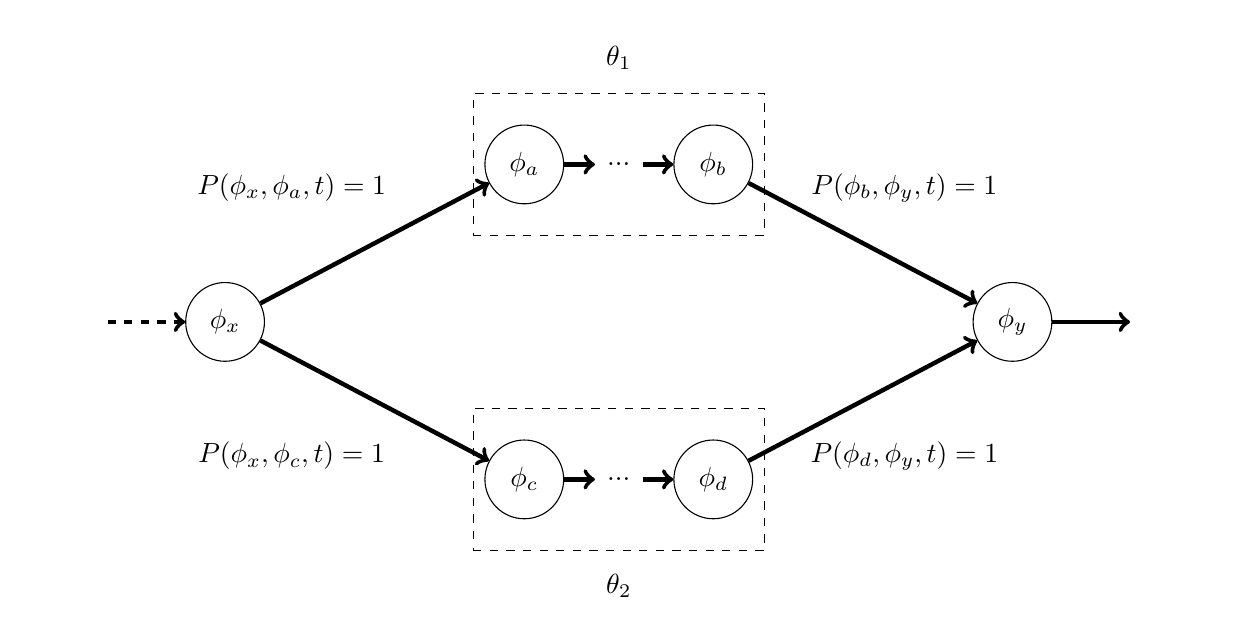
\begin{tikzpicture}
		
		
		\node[circle,draw=white,minimum width = 1cm] 
		(start) at (-2,0) {};
		
		\node[circle,draw=white,minimum width = 1cm] 
		(end) at (12,0) {};
		
		\node[circle, draw, minimum width = 1cm]        					   
		(branchStartNode) at (0,0) {$\phi_x$};
		
		\node[circle, draw, minimum width = 1cm]        					   
		(branchEndNode) at (10,0) {$\phi_y$};
		
		
		\node[circle, draw, minimum width = 1cm]        					   
		(Node1) at (3.8,2) {$\phi_a$};
		
		\node[circle, minimum width = 0.3cm]       					   
		(Node2) at (5,2) {...};
		
		\node[circle, draw, minimum width = 1cm]       					   
		(Node3) at (6.2,2) {$\phi_b$};
		
		\node[circle, draw, minimum width = 1cm]       					   
		(Node4) at (3.8,-2) {$\phi_c$};
		
		\node[circle, minimum width = 0.3cm]       					   
		(Node5) at (5,-2) {...};
		
		\node[circle, draw, minimum width = 1cm]       					   
		(Node6) at (6.2,-2) {$\phi_d$};
		
		\draw[ultra thick,->] (branchStartNode) edge node[xshift=-30 ,yshift=20]{$P(\phi_x,\phi_a, t) = 1$} (Node1);
		
		\draw[ultra thick,->] (branchStartNode) edge node[xshift=-30 ,yshift=-20]{$P(\phi_x,\phi_c, t) = 1$} (Node4);
		
		\draw[ultra thick,->] (Node3) edge node[xshift=15 ,yshift=20]{$P(\phi_b,\phi_y, t) = 1$} (branchEndNode);
		
		\draw[ultra thick,->] (Node6) edge node[xshift=15 ,yshift=-20]{$P(\phi_d,\phi_y, t) = 1$} (branchEndNode);
		
		% Dashed lines
		
		\draw[dashed,ultra thick, ->] (start) -- (branchStartNode);
		
		\draw[ultra thick, ->] (branchEndNode) -- (end);
		
		\draw[ultra thick, ->] (Node1) -- (Node2);
		
		\draw[ultra thick, ->] (Node2) -- (Node3);
		
		\draw[ultra thick, ->] (Node4) -- (Node5);
		
		\draw[ultra thick, ->] (Node5) -- (Node6);
		
		% Frames
		
		\node[rectangle, draw, dashed, minimum width =3.7cm, minimum height=1.8cm] (sub1) at (5,2) {};
		\node[circle,above of=sub1, yshift=10] (label1) {$\theta_1$};
		
		\node[rectangle, draw, dashed, minimum width =3.7cm, minimum height=1.8cm] (sub2) at (5,-2) {};
		\node[circle,below of=sub2, yshift=-10] (label2) {$\theta_2$};
		
	\end{tikzpicture}
	\caption{Parallel structure in a serverless workflow.}
\end{figure}

Clearly, the response time of a parallel structure is equal to the longest response time of all its sub-choreographies.

Formally, let $\theta_i \in \Theta$ the $i$-th sub-choreography of $\mathcal{P}$, where $i \in \N \cap \left[1,n\right]$, and $\textbf{x}_{\mathcal{C}} \in \textbf{X}_{\mathcal{C}}$ a choreography configuration.

At any time $t$, the average response time and billed cost of $\mathcal{P}$ can be computed as follows:

\begin{equation}
	RT(\mathcal{P},\textbf{x}_{\mathcal{C}}, t) \mathDef max \left\lbrace RT(\theta_i,\textbf{x}_{\mathcal{C}}, t) \mid \theta \in \Theta \right\rbrace 
\end{equation}

\begin{equation}
	C(\mathcal{P},\textbf{x}_{\mathcal{C}}, t) \mathDef \sum_{i = 1}^n C(\theta_i,\textbf{x}_{\mathcal{C}}, t)
\end{equation}

Since, by definition, we imposed that all sub-choreography of $\mathcal{P}$ have exit probability equal to zero, the exit probability of the a parallel structure is zero too. Therefore, formally:

\begin{equation}
	P_{exit}(\mathcal{P}, t) = 0
\end{equation}

\subsection{Conditional Loop}

Any structure $\mathcal{L} = (\Phi',E',\Theta)$ such that:

\begin{eqnarray}
	\omega(\mathcal{L}) \in \Omega(\mathcal{L}) \\
	\mathscr{T}(\alpha(\mathcal{L})) = \mathscr{T}(\phi_x) = \tau_{\alpha} \\ \mathscr{T}(\omega(\mathcal{L})) = \mathscr{T}(\phi_y) = \tau_{\omega} \\
	|\Theta| = 1  & \\
	|succ(\alpha(\mathcal{P}))| = 2 \\
	|prev(\alpha(\mathcal{P}))| \leq 2 \\
	|prev(\omega(\mathcal{P}))| = 1 \\
	E[I_{\theta}] \geq 0 & \qquad \theta \in \Theta \\
	P(\phi_{x}, \alpha(\theta), t) = x & \\
	P(\phi_{x}, \phi_{y},t) = 1 - x & \\
	P(\omega(\theta), \phi_{x},t) = 1 & \qquad \theta \in \Theta \\
	P(\phi_x, \alpha(\theta),t) + P(\phi_{x}, \phi_{y},t) = 1 & \qquad \theta \in \Theta
\end{eqnarray}

is called \textit{conditional loop structure} and $\tau$ denotes a \textit{conditional loop} type; it is used to model a \texttt{while} and \texttt{for} programming structures inside a serverless application. 

\begin{figure}
	\centering
	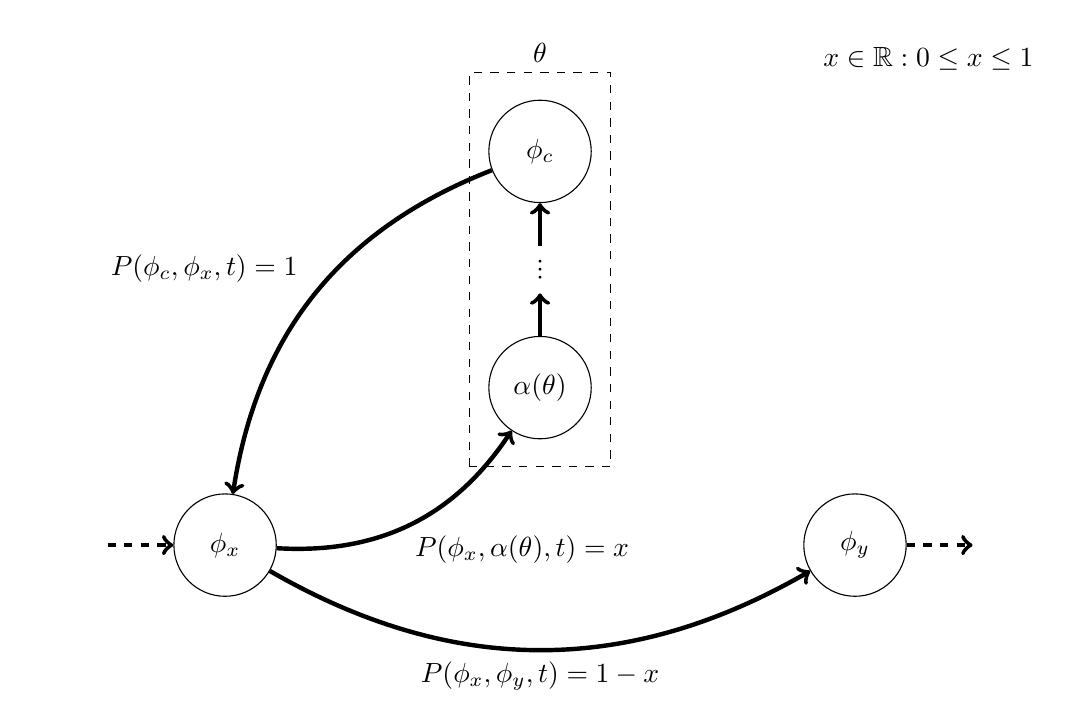
\begin{tikzpicture}
		
		
		\node[circle,draw=white,minimum width = 1cm] 
		(start) at (-2,0) {};
		
		\node[circle,draw=white,minimum width = 1cm] 
		(end) at (10,0) {};
		
		\node[circle, draw, minimum width = 1.3cm]        					   
		(startLoopNode) at (0,0) {$\phi_x$};
		
		\node[circle, draw, minimum width = 1.3cm]        					   
		(endLoopNode) at (8,0) {$\phi_y$};
		
		\node[circle, draw, minimum width = 1.3cm]        					   
		(node1) at (4,2) {$\alpha(\theta)$};
		
		\node[circle, minimum width = 0.5cm, rotate=90]        					   
		(node2) at (4,3.5) {...};
		
		\node[circle, draw, minimum width = 1.3cm]        					   
		(node3) at (4,5) {$\phi_c$};
		
		% Edges...
		
		\draw[bend right,below, ultra thick,->] (startLoopNode) edge node[xshift=40]{$P(\phi_x,\alpha(\theta),t) = x$} (node1);
		
		\draw[bend right,above, ultra thick,->] (node3) edge node[xshift=-40]{$P(\phi_c,\phi_x,t) = 1$} (startLoopNode);
		
		\draw[bend right,below, ultra thick,->] (startLoopNode) edge node[]{$P(\phi_x,\phi_y,t) = 1 - x$} (endLoopNode);
		
		
		
		\draw[dashed,ultra thick, ->] (start) -- (startLoopNode);
		\draw[dashed,ultra thick, ->] (endLoopNode) -- (end);
		
		
		\draw[ultra thick, ->] (node1) -- (node2);
		\draw[ultra thick, ->] (node2) -- (node3);
		
		% Frames
		
		\node[rectangle, draw, dashed, minimum width =1.8cm, minimum height=5cm] (sub1) at (4,3.5) {};
		\node[circle,above of=sub1, yshift=50] (label1) {$\theta$};
		
		%legend
		
		\matrix [below left] at (current bounding box.north east) {
			\node [] {$x \in \mathbb{R} : 0 \leq x \leq 1$}; \\
		};
		
	\end{tikzpicture}
	\caption{Conditional loop structure in a serverless workflow.}
\end{figure}

Similarly to the branch structure, we have adopt the equation \ref{naiveProbability} to compute the transition probability $P(\phi_{x}, \alpha(\theta), t)$.

In order to compute performance data of a loop structure, $E[I_{\theta}(t)]$, that is the expected value of the number of iterations of $\mathcal{L}$ at the time $t$, is required.

To compute aforementioned information, we can model our problem using geometric distribution, which gives the probability according to which the first occurrence of success requires $k \in \N$ independent trials, each with success probability $p$ and failure probability $q = 1 - p$. In our case, if the our success corresponds to event ``\textit{we will not execute the loop body}", we know that success probability $p$ is given by:

\begin{eqnarray}
	p = P(\phi_x,\phi_y,t) = 1 - P\Big(\phi_{x}, \alpha(\theta),t\Big)
\end{eqnarray}

Then:

\begin{eqnarray}
	P(I_{\theta} = k) & = & p \cdot (1-p)^{k-1} \nonumber \\
	& = & pq^{k-1} \nonumber \\
	& = & \Big[  1 - P\Big(\phi_{x}, \alpha(\theta),t\Big) \Big] \cdot \bigg[  P\Big(\phi_{x}, \alpha(\theta),t\Big) \bigg] ^{k-1}
\end{eqnarray}

At any time $t$, the expected value regarding the number of iterations of $\mathcal{L}$, involving the execution of the sub-choreography $\theta$, can be computed as follows:

\begin{eqnarray}
	E[I_{\theta}(t)] & = & \sum_{k = 1}^\infty (k-1) pq^{k-1} \nonumber \\
	& = & p \sum_{k = 0}^\infty kq^{k} \nonumber \\
	& = & p \cdot \frac{q}{(1-q)^2} \nonumber \\
	& = & \dfrac{q}{p} \nonumber \\
	& = & \dfrac{P\Big(\phi_{x}, \alpha(\theta),t\Big)}{1 - P\Big(\phi_{x}, \alpha(\theta),t\Big)} 
\end{eqnarray}

At any time $t$, the response time and the cost of the conditional loop structure $\mathcal{L}$ can be computed as follows:

\begin{equation}
	RT(\mathcal{L},\textbf{x}_{\mathcal{C}}, t) \mathDef E[I_{\theta}(t)] \cdot RT(\theta_i,\textbf{x}_{\mathcal{C}}, t)
\end{equation}

\begin{equation}
	C(\mathcal{L},\textbf{x}_{\mathcal{C}}, t) \mathDef E[I_{\theta}(t)] \cdot C(\theta_i,\textbf{x}_{\mathcal{C}}, t)
\end{equation}

The exit probability of a conditional loop structure was been modeled, once again, exploiting the geometric distribution with success probability equal to $P_{exit}(\theta, t)$. To be precise, exit probability is modeled as the probability that the termination of the execution of the choreography to which $\mathcal{L}$ belongs requires $\lfloor E[I_{\theta}(t)] \rfloor$  executions of $\mathcal{L}$. Formally:

\begin{eqnarray}
	P_{exit}(\mathcal{L}, t) & \mathDef & \Big(1 -P_{exit}(\theta, t)  \Big)^{\lfloor E[I_{\theta}(t)] \rfloor - 1} \cdot P_{exit}(\theta, t)
\end{eqnarray}

\subsection{Branch}

Any structure $\mathcal{B} = (\Phi',E',\Theta)$ such that:

\begin{eqnarray}
	\mathscr{T}(\alpha(\mathcal{B})) = \mathscr{T}(\phi_x) = \tau_{\alpha} \\ \mathscr{T}(\omega(\mathcal{B})) = \mathscr{T}(\phi_y) = \tau_{\omega} \\
	|succ(\alpha(\mathcal{P}))| \geq 2 \\
	|prev(\omega(\mathcal{P}))| \leq |succ(\alpha(\mathcal{P}))| \\
	|\Theta| = n  & \qquad n \in \N \setminus \left\{0\right\} \\
	P(\phi_x, \alpha(\theta_i),t) \leq 1 & \qquad \forall i \in \SetFromOneTo{n} \\
	\sum_{i = 1}^n P(\phi_x, \alpha(\theta_i),t) = 1 & \\
	E[I_{\theta}] = 1 & \qquad \forall \theta \in \Theta \\
\end{eqnarray}

is called \textit{branch structure} and $\tau$ denotes a \textit{branch} type. More precisely, if $|\Theta| = 2$, $\mathcal{B}$ will be called \textit{if-else-branch structure}; if $|\Theta| = 2$, $\mathcal{B}$ will be called \textit{switch-branch structure}. When $|\Theta| = 1$ and $(\phi_x,\phi_y) \in E$, $\mathcal{B}$ is called \textit{if-branch structure}. Clearly, it is used to model \texttt{if}, \texttt{if-else} and \texttt{switch} programming structures inside a serverless application. It is not necessary that $\omega(\mathcal{B})$ exists.

\begin{figure}
	\centering
	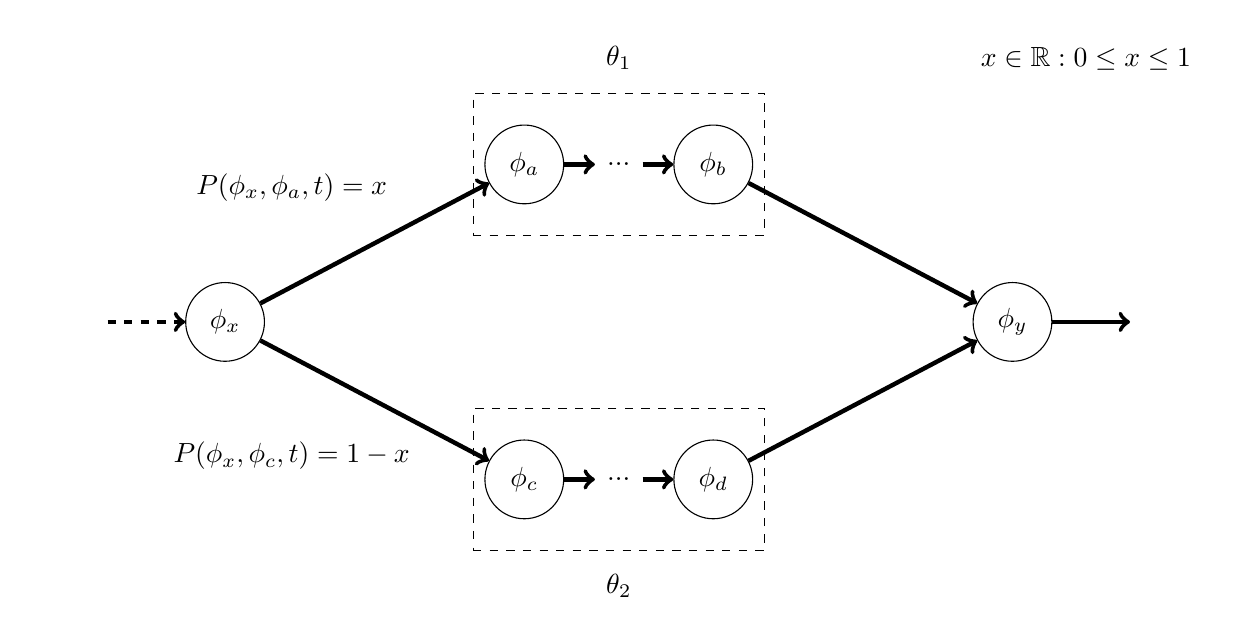
\begin{tikzpicture}
		
		
		\node[circle,draw=white,minimum width = 1cm] 
		(start) at (-2,0) {};
		
		\node[circle,draw=white,minimum width = 1cm] 
		(end) at (12,0) {};
		
		\node[circle, draw, minimum width = 1cm]        					   
		(branchStartNode) at (0,0) {$\phi_x$};
		
		\node[circle, draw, minimum width = 1cm]        					   
		(branchEndNode) at (10,0) {$\phi_y$};
		
		
		\node[circle, draw, minimum width = 1cm]        					   
		(Node1) at (3.8,2) {$\phi_a$};
		
		\node[circle, minimum width = 0.3cm]       					   
		(Node2) at (5,2) {...};
		
		\node[circle, draw, minimum width = 1cm]       					   
		(Node3) at (6.2,2) {$\phi_b$};
		
		\node[circle, draw, minimum width = 1cm]       					   
		(Node4) at (3.8,-2) {$\phi_c$};
		
		\node[circle, minimum width = 0.3cm]       					   
		(Node5) at (5,-2) {...};
		
		\node[circle, draw, minimum width = 1cm]       					   
		(Node6) at (6.2,-2) {$\phi_d$};
		
		\draw[ultra thick,->] (branchStartNode) edge node[xshift=-30 ,yshift=20]{$P(\phi_x,\phi_a, t) = x$} (Node1);
		
		\draw[ultra thick,->] (branchStartNode) edge node[xshift=-30 ,yshift=-20]{$P(\phi_x,\phi_c, t) = 1-x$} (Node4);
		
		\draw[ultra thick,->] (Node3) edge (branchEndNode);
		
		\draw[ultra thick,->] (Node6) edge (branchEndNode);
		
		% Dashed lines
		
		\draw[dashed,ultra thick, ->] (start) -- (branchStartNode);
		
		\draw[ultra thick, ->] (branchEndNode) -- (end);
		
		\draw[ultra thick, ->] (Node1) -- (Node2);
		
		\draw[ultra thick, ->] (Node2) -- (Node3);
		
		\draw[ultra thick, ->] (Node4) -- (Node5);
		
		\draw[ultra thick, ->] (Node5) -- (Node6);
		
		% Frames
		
		\node[rectangle, draw, dashed, minimum width =3.7cm, minimum height=1.8cm] (sub1) at (5,2) {};
		\node[circle,above of=sub1, yshift=10] (label1) {$\theta_1$};
		
		\node[rectangle, draw, dashed, minimum width =3.7cm, minimum height=1.8cm] (sub2) at (5,-2) {};
		\node[circle,below of=sub2, yshift=-10] (label2) {$\theta_2$};
		
		legend
		
		\matrix [below left] at (current bounding box.north east) {
			\node [] {$x \in \mathbb{R} : 0 \leq x \leq 1$}; \\
		};
		
		
	\end{tikzpicture}
	\caption{An if-else-branch structure in a serverless workflow}
\end{figure}

Since any branch have the same possibility of be traversed during different execution of $\mathcal{B}$, we have adopted naive probability to model transition probabilities. Formally:

\begin{equation}\label{naiveProbability}
	P(\phi_x, \alpha(\theta),t) = \dfrac{|I_{\theta}(t)|}{|I_{\mathcal{B}}(t)|} \qquad \forall \theta \in \Theta
\end{equation}

where $|I_{\theta}|$ ($|I_{\mathcal{B}}|$) denotes how many times the sub-choreography $\theta$ (structure $\mathcal{B}$) was been executed in the past at time $t$.

Let $\theta_i \in \Theta$ the $i$-th sub-choreography of $\mathcal{B}$, where $i \in \N \cap \left[1,n\right]$. At any time $t$, the response time and the cost of the branch structure $\mathcal{B}$ can be computed as follows:

\begin{equation}
	RT(\mathcal{B},\textbf{x}_{\mathcal{C}}, t) \mathDef \sum_{i = 1}^n P(\phi_{x}, \alpha(\theta_i),t) \cdot  RT(\theta_i,\textbf{x}_{\mathcal{C}}, t)
\end{equation}

\begin{equation}
	C(\mathcal{B},\textbf{x}_{\mathcal{C}}, t) \mathDef \sum_{i = 1}^n P(\phi_{x}, \alpha(\theta_i),t) \cdot C(\theta_i,\textbf{x}_{\mathcal{C}}, t)
\end{equation}

The exit probability of a branch structure can be computed as follows:

\begin{equation}
	P_{exit}(\mathcal{B}, t) \mathDef \sum_{i = 1}^n P(\phi_{x}, \alpha(\theta_i),t) \cdot P_{exit}(\theta_i, t)
\end{equation}

\section{Performance Evaluation of Concrete Functions}

Clearly, in order to select an appropriate serverless choreography configuration able to effectively guarantee SLA requirements specified by users, we need firstly to evaluate the performance of concrete functions, in terms of average values regarding response time and charged costs.

However, to develop both an analytical way and a software framework capable to evaluate concrete serverless function performance, we first need to understand
how they are managed by FaaS platforms.

\subsection{FaaS Platform Modeling}

According to our model point of view, at any time $t$, any FaaS platform provider acts as a ``\textit{set}'' of $M/G/K(t)_{\textbf{C}_{max}}/K(t)_{\textbf{C}_{max}}$ queueing systems, also called \textit{$K(t)$-server loss systems}, where:

\begin{itemize}
	
	\item $\textbf{C}_{max} \in \N \setminus \left\{0\right\}$ is a scalar representing the queuing system's concurrency limit.
	
	In other words, $\textbf{C}_{max}$ is the maximum size of the warm pool, therefore it represents the maximum number of function instances being in running state simultaneously at time $t$. 
	
	Please note that $\textbf{C}_{max}$ not necessary coincide with a global concurrency limit because it can represents a local concurrency limit too. We will give more details about this very soon.
	
	\item At any time $t \geq 0$, there are $K(t)$ function instances. Since each instance can process only one request, we can say that the system has capacity for $K(t)$ invocation requests in total. The number of function instance, and consequently system's capacity, can change over time. 
	
	At any time $t$, following condition must be hold:
	
	\begin{equation}
		0 \leq K(t) \leq {C}_{\textbf{max}}
	\end{equation}
	
	\item Since no queue is involved, if the maximum concurrency level is reached, that is $K(t) = {C}_{\textbf{max}}$, any incoming request at time $t$, that sees all $K(t)$ function instances in running state, will be permanently dropped \footnote{Indeed, a queue exists; there are previous studies stating that all FaaS platform providers adopt a scheduling policies based on \textit{first-come-first-served} (FIFO) algorithms. Anyways, since the built of a QoS-aware scheduler is out of the scope of this dissertation, in order to meet QoS objectives, we have decided to drop any request exceeding maximum concurrency level instead of relying on scheduling policies provided by FaaS platforms.}.
	
	\item No priority is considered among incoming request.
	
	\item Service times have a general distribution while a Poisson arrival process is assumed.
\end{itemize} 

\begin{figure}[h!]
	\centering
	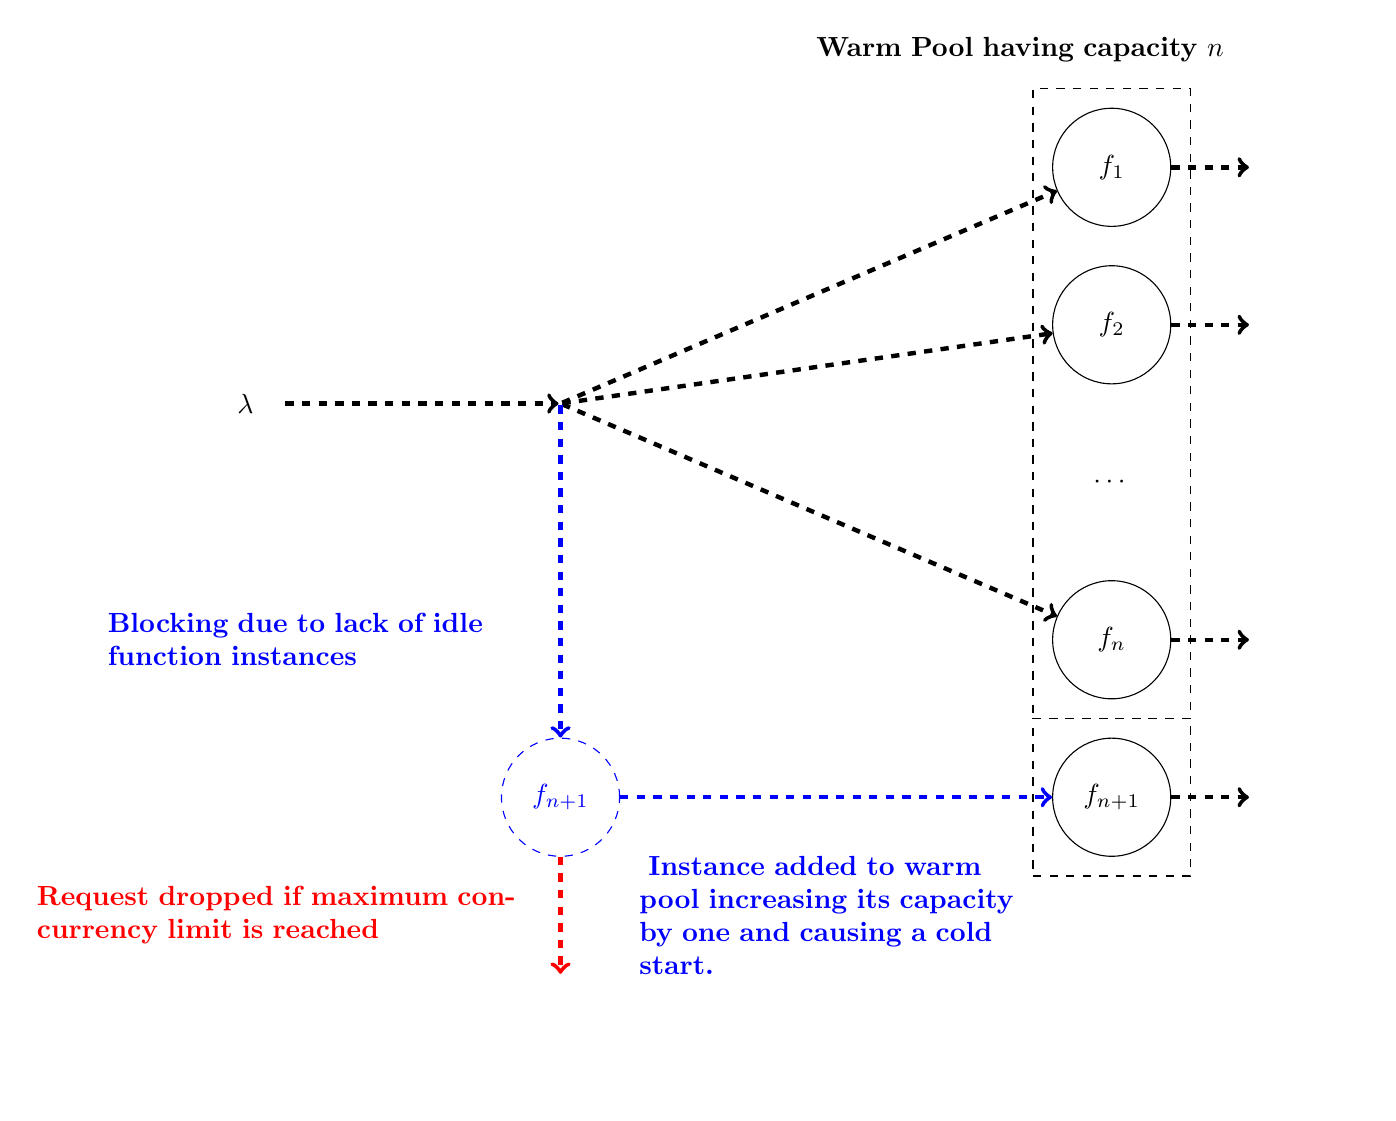
\begin{tikzpicture}
		
		
		\node[circle, minimum width = 1cm]        					   
		(startNode) at (-8,0) {$\lambda$};
		
		\node[circle, inner sep=0pt]        					   
		(startNode2) at (-4,0) {};
		
		% Node
		
		\node[circle, draw, minimum width = 1.5cm]        					   
		(f1) at (3,3) {$f_1$};
		\node[circle, draw, minimum width = 1.5cm]       					   
		(f2) at (3,1) {$f_2$};
		\node[circle, minimum width = 1.5cm]       					   
		(fxxx) at (3,-1) {$\cdots$};
		\node[circle, draw, minimum width = 1.5cm]       					   
		(fn) at (3,-3) {$f_n$};
		\node[circle, draw, minimum width = 1.5cm]       					   
		(fn2) at (3,-5) {$f_{n+1}$};
		
		\node[circle, dashed, blue, draw, minimum width = 1.5cm]       					   
		(fn2fake) at (-4,-5) {$f_{n+1}$};
		
		\node[circle, dashed, minimum width = 1.5cm]       					   
		(fn2fakeExit) at (-4,-8) {};
		
		% Exit node
		
		\node[circle, minimum width = 1.5cm]        					   
		(Ef1) at (5.5,3) {};
		\node[circle, minimum width = 1.5cm]       					   
		(Ef2) at (5.5,1) {};
	

		\node[circle, minimum width = 1.5cm]       					   
		(Efn) at (5.5,-3) {};
		\node[circle, minimum width = 1.5cm]       					   
		(Efn2) at (5.5,-5) {};
		
	
		% EDGE
	
		\draw[dashed, ultra thick,->] (startNode) -- (startNode2);
		\draw[dashed, ultra thick,->] (startNode2) -- (f1);
		\draw[dashed, ultra thick,->] (startNode2) -- (f2);
		\draw[dashed, ultra thick,->] (startNode2) -- (fn);
		\draw[dashed, ultra thick,->,blue] (fn2fake) -- (fn2);
		\draw[dashed, ultra thick,->, blue] (startNode2) -- (fn2fake);
		
		% Exit EDGE
		
		\draw[dashed, ultra thick,->] (f1) -- (Ef1);
		\draw[dashed, ultra thick,->] (f2) -- (Ef2);
		\draw[dashed, ultra thick,->] (fn) -- (Efn);
		\draw[dashed, ultra thick,->] (fn2) -- (Efn2);
		\draw[dashed, ultra thick,->,red] (fn2fake) -- (fn2fakeExit);
		
		%\node[circle,below of=sub1, yshift=10] (label1) {$\theta_1$};
		\node[rectangle, draw, dashed, minimum width =2cm, minimum height=2cm] (sub1) at (3,-5) {};
		
		\node[rectangle, draw, dashed, minimum width =2cm, minimum height=8cm] (sub1) at (3,0) {};
		
		%\draw[ultra thick,->] (ParNode1) edge node[xshift=15 ,yshift=15]{$P(\phi_2,\phi_4) = 1$} (ParEndNode);
		%\draw[ultra thick,->] (ParNode2) edge node[xshift=15 ,yshift=-15]{$P(\phi_3,\phi_4) = 1$} (ParEndNode);
		
		%\draw[dashed,ultra thick, ->] (start) -- (ParStartNode);
		%\draw[dashed,ultra thick, ->] (ParEndNode) -- (end);
		
		
		\node[text width=6.5cm] at (2.5,4.5) {\textbf{Warm Pool having capacity} $n$};
		
		\node[text width=5cm, blue] at (-0.5,-6.5) {\textbf{ Instance added to warm pool increasing its capacity by one and causing a cold start.}};
		
		\node[text width=5.5cm, blue] at (-7,-3) {\textbf{Blocking due to lack of idle function instances}};
		
		\node[text width=6.3cm, red] at (-7.5,-6.5) {\textbf{Request dropped if maximum concurrency limit is reached}};
		
	\end{tikzpicture}
	\caption{An overview of the proposed system model using $M/G/K(t)_{\textbf{C}_{max}}/K(t)_{\textbf{C}_{max}}$ queening systems.}
\end{figure}

\subsection{Concrete Function Swarm}

To complete the formalization of our model and understand how concrete function performances are evaluated, it is necessary to introduce another very important concept to make our model compatible with all concurrency limit models adoptable by FaaS providers.

Let $l \in \N$, $R$ a resource owner, $P$ a serverless computing platform provider and $\Omega_{P_R}$ the set of all concrete serverless functions hosted on $P$ belonging to $R$.

A \textit{concrete function swarm}, or simply \textit{swarm}, is the set $\omega_{P_R}^{(l)} \subseteq \Omega_{P_R}$ containing all concrete functions sharing the same limit $l$ in term of the max number of serverless function instance runnable at the same time by $P$; in that case, we call $l$ as \textit{swarm's concurrency limit}.

In simple terms, only at most $l$ executions of any concrete functions belonging to $\omega_{P_R}^{(l)}$ can be performed simultaneously by $P$. The value of $l$ depends on the concurrency model adopted by $P$. 

\begin{itemize}
	
	\item If $P$ imposed a \textit{per-function} limit, then $|\omega_{P_{R_l}}| = 1$, that is, $\omega_{P_R}^{(l)}$ contains only one function and $l$ will represent the provider's per-function limit. 
	
	In that case, a dedicated $M/G/K(t)_{l}/K(t)_{l}$ queuing system corresponds to each concrete function belonging to $\omega_{P_R}^{(l)}$, which will serve all invocation request regarding only its corresponding concrete function.  
	
	\item If $P$ imposed a \textit{per-account} limit, then $\omega_{P_R}^{(l)} = \Omega_{P_R}$, that is the swarm includes all concrete function deployed on $P$ by $R$, while $l$ represents the provider's global concurrency limit. 
	
	In that case, there is only one $M/G/K(t)_{l}/K(t)_{l}$ queuing system serving all invocation requests regarding any concrete function belonging to $\Omega_{P_R}$. 

\end{itemize}

From now, the sets $\omega_{P_R}^{(l)}$ and $\Omega_{P_R}$ will be briefly and respectively denoted by $\omega_{P}^{(l)}$ and $\Omega_{P}$ when no confusion can arise about the resource owner $R$. Moreover, we will adopt $\textbf{Q}_{\omega_{P}^{(l)}}$ notation to refer to the $M/G/K(t)_{l}/K(t)_{l}$ queuing system serving all invocation requests of any concrete function belonging to $\omega_{P}$. 

\subsubsection{Cold Start Probability}

According to our model, if maximum concurrency level is not exceeded, the rejection of a request by the warm pool will trigger a cold start, adding a new function instance to the warm pool in order to handle aforementioned request. 

Now we have to estimate the probability according to which a request is rejected by the warm pool; in other words, we must to compute the \textit{cold start probability}. 

Formally, let $l \in \N$, $P$ a serverless computing platform provider, $\omega_{P}^{(l)}$ a swarm and $\textbf{Q}_{\omega_{P}^{(l)}}$ its corresponding queuing system on the FaaS platform provider. Following functions will be used:

\begin{itemize}
	\item $R(\textbf{Q}_{\omega_{P}^{(l)}}, t)$ representing the function returning the number of running state function instances at time $t$ on $\textbf{Q}_{\omega_{P}^{(l)}}$.
	
	\item $K(\textbf{Q}_{\omega_{P}^{(l)}}, t)$ returning instead the number of function instances at time $t$ deployed on $\textbf{Q}_{\omega_{P}^{(l)}}$.
\end{itemize}

In this section, to simplify our notations, since no confusion can arise about the queuing system, $R(\textbf{Q}_{\omega_{P}^{(l)}}, t)$ will be briefly denoted as $R(t)$ and $K(\textbf{Q}_{\omega_{P}^{(l)}}, t)$ as $K(t)$.

When a new invocation request of any function belonging to $\omega_{P}^{(l)}$ arrives on $\textbf{Q}_{\omega_{P}^{(l)}}$, one of the following events can occur:

\begin{itemize}
	\item If $K(t_n) < l$ and $R(t_n) < K(t_n)$, that is the number of function instances into the warm pool is less than the swarm maximum concurrency level and there are some function instance in idle state, a warm start will occur, resulting that $R(t_{n+1}) = R(t_n) + 1$.
	
	
	\item If $K(t_n) < l$ and $R(t_n) = K(t_n)$, that is the number of function instances into the warm pool is once again less than the swarm maximum concurrency level but there is no function instance in idle state, a cold start will occur and the size of the warm pool will be increased by one, that is $K(t_{n+1}) = K(t_n) + 1$.
	
	The accepted request will be managed by the newly spinned up function instance, causing that $R(t_{n+1}) = R(t_n) + 1$.
	
	\item If $K(t) = R(t) = l$, that is the warm pool reaches its maximum possible size according to FaaS policies, aforementioned request will be rejected.
\end{itemize}

If at time $t_n$ a concrete function execution has been completed, that event will cause $R(t_{n+1}) = R(t_n) - 1$. 

Conversely, if a function instance has not  received any request during the last expiration threshold units of time, it will expire causing the decreasing of warm pool size, that is $K(t_{n+1}) = K(t_n) - 1$.

Finally, at any time $t$, the \textit{cold start probability} $\textbf{P}_{\omega_{P_R}^{(l)}}(t)$ referring to the invocations of any function belonging to the swarm $\omega_{P_R}^{(l)}$, can be formally defined as the probability that an arrival request of invocation finds all function instances of the warm pool busy; using Erlang-B formula, that probability can be calculated as follows:

\begin{equation}\label{er}
	\displaystyle \textbf{P}_{\omega_{P_R}^{(l)}}(t) = \dfrac{\rho(t)^{K(t)}}{K(t)!} \cdot \Bigg( \displaystyle\sum_{j=0}^{K(t)} \dfrac{\rho(t)^j}{j!}\Bigg)^{-1}
\end{equation}

where:

\begin{itemize}
	
	\item $\displaystyle \rho(t) = \frac{\lambda(t)}{\mu_{w}}$ represents system utilization or load of the warm pool at time $t$ where:
	
	\begin{itemize}
		
		\item $\lambda(t)$ represents the \textit{average arrival rate} at time $t$, that is the rate at which invocation requests, regarding serverless concrete functions belonging to $\omega_{P_R}^{(l)}$, arrive to our system. It is expressed in $invocations \cdot s^{-1}$.
				
		Since arrival rate varies during the day, $\lambda(t)$ must be estimated at runtime, over multiple time intervals spent observing our system.
		
		We adopt the exponential moving average based approach to compute an estimation of $\lambda(t)$. Periodically, at any time $t$, our framework computes the number $Y_t$ of all received invocation requests for any function belonging to $\omega_{P_R}^{(l)}$ within last second. Then $\lambda(t)$ is estimated as follows:
		
		\begin{equation}
			\lambda(t) \mathDef
			\begin{cases}
				Y_o & \text{if}\ t = 0\\ 
				\alpha \cdot Y_t + (1 - \alpha) \cdot \lambda(t-1) & \text{if}\ t > 0\\
				
			\end{cases}\,.
		\end{equation}
		
		\item $\mu_{w} = E[S_w]$ represents the \textit{warm start average service rate}, that is the rate at which executions requests are served when a warm start occurs, while $E[S_w]$ is the \textit{warm start average time}, which is the average time required to complete aforementioned request.
		
	\end{itemize}
	
\end{itemize}

Finally, in order to simplify the calculation of the expression \ref{er}, according to \cite{ERLANG}, it can be expressed  recursively as follows:

\begin{eqnarray}
	\dfrac{1}{B(\rho(t),0)} & = & 1 \\
	\dfrac{1}{B(\rho(t),i)} & = & 1 + \dfrac{i}{\rho(t)} \cdot \dfrac{1}{B(\rho(t),i-1)} \qquad \forall j \in \SetFromOneTo{K(t)} \\
\end{eqnarray}

where:

\begin{equation}
	B(\rho(t),i) \mathDef \dfrac{\rho(t)^{i}}{i!} \cdot \Bigg( \displaystyle\sum_{j=0}^{i} \dfrac{\rho(t)^j}{j!}\Bigg)^{-1}
\end{equation}

\subsubsection{Choreography Swarm}

Let $\mathcal{C} = (\Phi,E)$ a choreography, to build its configuration $\textbf{x}_{\mathcal{C}}$, we first need to identify all swarms corresponding to each concrete function $f_{\phi} \in \textbf{F}_{\phi}$, for all $\phi \in \mathscr{F_E}$, because we have to check if we can execute all concrete functions specified in $\textbf{x}_{\mathcal{C}}$, without exceeding maximum concurrency level on each FaaS platforms where aforementioned functions will be executed.

Informally, a \textit{choreography swarm} $\widetilde{\textbf{S}}_{\mathcal{C}}$ represents the set of all swarms corresponding to all concrete functions used by $\mathcal{C}$. 

Formally, let $m \in \N$ the total number of FaaS platform providers where at least one concrete function is deployed by a given resource owner, a choreography swarm can be defined as follows:

\begin{equation}
	\widetilde{\textbf{S}}_{\mathcal{C}} \mathDef \left\{ \omega_{P}^{(l)} \in \bigcup_{i=1}^n \Omega_{P_i} : \exists f_{\phi} \in \omega_{P}^{(l)} \text{ such that } f_{\phi} \in \textbf{F}_{\phi}, \forall \phi \in \mathscr{F_E}(\mathcal{C}) \right\}
\end{equation}

Please note that, let $\mathcal{C}_1 = (\Phi_1,E_1)$ and $\mathcal{C}_2 = (\Phi_2,E_2)$ two different choreographies belonging to the same resource owner, it is generally verified that:

\begin{equation}
	\widetilde{\textbf{S}}_{\mathcal{C}_1} \cap \widetilde{\textbf{S}}_{\mathcal{C}_2} \neq \emptyset
\end{equation}

that is a swarm can be shared by multiple choreographies, therefore any implementation of our model has to pay attention on possible race conditions. 

Finally, we will use following function:

\begin{equation}
	N(\mathcal{C},\textbf{x}_{\mathcal{C}},\omega_{P}^{(l)}) = \sum_{x_{\phi} \in \textbf{x}_{\mathcal{C}}} \sum_{\substack{f_{\phi} \in x_{\phi} \\ f_{\phi} \in \omega_{P}^{(l)}}} 1
\end{equation}

that is, $N(\mathcal{C},\textbf{x}_{\mathcal{C}},\omega_{P}^{(l)},t)$ denotes the number of concrete functions used in $\textbf{x}_{\mathcal{C}}$ 


\subsection{Concrete Function Performance Computation}

Finally, we can introduce how concrete function performance can be computed according to our model.

Let $x_{\phi} = (f_{\phi},m)$ an executable function configuration such that $f_{\phi} \in \omega_{P_R}^{(l)} \subset \textbf{F}_{\phi}$ represents a concrete function implementing the executable function $\phi \in \mathscr{F_E}(\mathcal{C})$ and belonging to the swarm $\omega_{P_R}^{(l)}$, where $l \in \N$ is its concurrency limit. Moreover, $m \in \textbf{M}_{f_{\phi}} \subseteq \N$ denotes the value of the memory size selected by our framework for the execution of $f_{\phi}$.

Let's define following functions:

\begin{itemize}	
	\item $C : \textbf{F}_{\phi} \times \textbf{M}_{f_{\phi}} \times \mathbb{R}^+ \to \mathbb{R}^+$ is the \textit{cost function} for any serverless concrete functions belonging to the implementation-set $\textbf{F}_{\phi}$. 
	
	It returns the \textit{average cost} paid by users when $f_{\phi}$ is executed using an allocated memory size equal to $m$ at time $t$. 
		
	It can be defined as follows:
	
	\begin{eqnarray}
		C(x_{\phi},t) & \mathDef & C(f_{\phi},m,t) \nonumber \\
		& = & C_{avg}^{(c)}(f_{\phi}, m,t) \cdot \textbf{P}_{\omega_{P_R}^{(l)}}(t) + \\
		& & \qquad C_{avg}^{(w)}(f_{\phi}, m,t) \cdot \Big( 1 - \textbf{P}_{\omega_{P_R}^{(l)}}(t)  \Big) \nonumber
	\end{eqnarray}
	
	where:
	
	\begin{itemize}
		\item At any time $t$. when $f_{\phi}$ is executed with an allocated memory size equal to $m$, 
		$C_{avg}^{(c)}(f_{\phi}, m,t)$ represents the average cost paid when a cold start is occurred while, conversely, $C_{avg}^{(w)}(f_{\phi}, m,t)$ represents the average cost paid in case of warm start.
	\end{itemize}
	
	
	\item $RT : \textbf{F}_{\phi} \times \textbf{M}_{f_{\phi}} \times \mathbb{R}^+ \to \mathbb{R}^+$ is the \textit{delay function} for any serverless concrete functions belonging to the implementation-set $\textbf{F}_{\phi}$. 
	
	It returns the \textit{average response time} paid by users when $f_{\phi}$ is executed using an allocated memory size equal to $m$ at time $t$. 
	
	It can be defined as follows:
	
	\begin{eqnarray}
		RT(x_{\phi},t) & \mathDef & RT(f_{\phi},m,t) \nonumber \\
		& = & RT_{avg}^{(c)}(f_{\phi}, m,t) \cdot \textbf{P}_{\omega_{P_R}^{(l)}}(t) + \\ 
		& & \qquad RT_{avg}^{(w)}(f_{\phi}, m,t) \cdot \Big( 1 - \textbf{P}_{\omega_{P_R}^{(l)}}(t)  \Big) \nonumber
	\end{eqnarray}

	where:
	
	\begin{itemize}
		\item $RT_{avg}^{(c)}(f_{\phi}, m,t)$ represents the average response time occurred when a cold start is occurred and $RT_{avg}^{(w)}(f_{\phi}, m,t)$ is the one occurred in case of in case of warm start.
	\end{itemize}
\end{itemize}

Obviously, our framework has to determine $RT_{avg}^{(c)}(f_{\phi}, m,t)$, $RT_{avg}^{(w)}(f_{\phi}, m,t)$, $C_{avg}^{(c)}(f_{\phi}, m,t)$ and $C_{avg}^{(w)}(f_{\phi}, m,t)$ using time series data, containing historical performance data of $f_{\phi}$ under different memory configurations, collected by our logging framework. To compute aforementioned estimations, we adopt the exponential moving average based approach.

For instance, referring to the computation of $RT_{avg}^{(c)}(f_{\phi}, m,t)$, let $Y_t$ the response time of $f_{\phi}$ when it is executed with memory size $m$ at a given time $t$, following formula is used:

\begin{equation}
	RT_{avg}^{(c)}(f_{\phi}, m,t) \mathDef
	\begin{cases}
		Y_o & \text{if}\ t = 0\\ 
		\alpha \cdot Y_t + (1 - \alpha) \cdot \lambda(t-1) & \text{if}\ t > 0\\
		
	\end{cases}\,.
\end{equation}

\section{Executable Function Performance Evaluation}

In this section, we will describe how to evaluate the performance of any executable serverless function, in terms of average values regarding response time and charged costs, when it is executed. 

Supposing to have a choreography $\mathcal{C} = (\Phi,E)$, let $x_{\phi_{i_{j}}} = (f_j, m_j)$ an executable function configuration for $\phi_i \in \mathscr{F_E}(\mathcal{C})$, for some $i \in \N \cap [1,|\mathscr{F_E}(\mathcal{C})|]$ and $j \in \N \cap [1,|\textbf{F}_{\phi_{i}} \times \N|]$. In order to evaluate the performance of $\phi$, we have to introduce some useful notations and functions as follows:

\begin{itemize}
	\item For some $n \in \N$, $\widehat{\theta_k}^{(\phi_i)} \mathDef \left\{ \theta^{(\phi_i)}_1, \ldots, \theta^{(\phi_i)}_n \right\}$ represents the set of all sub-choreographies of $\mathcal{C}$ such that:
	
	\begin{equation}
		\phi_i \in \mathscr{F_E}(\theta^{(\phi_i)}_1)
	\end{equation}
	
	\begin{equation}
		\theta^{(\phi_i)}_n = \mathcal{C}
	\end{equation}
	
	\begin{equation}
		\theta^{(\phi_i)}_k = (\Phi_k, E_k) \text{ is a sub-choreography of } \theta^{(\phi_i)}_{k+1} \qquad \forall k \in \left[1;n-1\right]
	\end{equation}

	\item $E[I_{\phi_i}(t)]$ represents the expected value regarding the number of invocation of the executable function $\phi_i$ at time $t$, which can be defined as follows.
	
	\begin{equation}	
		E[I_{\phi_i}(t)] \mathDef \left\{
		\begin{array}{lcr}
			1 & \text{\textit{if}} & n = 1 \\ 
			\displaystyle \prod_{k = 2}^n E[I_{\theta_{k-1}^{(\phi_i)}}(t)] & \text{\textit{if}} & n \geq 2 \\
		\end{array} \right.
	\end{equation}
	
	\item $P_{exe}^C(\theta^{(\phi_i)}_k, t)$ is the probability to execute the entry point $\alpha(\theta^{(\phi_i)}_k)$ of the choreography $\theta^{(\phi_i)}_k$ when the function $pred(\alpha(\theta^{(\phi_i)}_k))$ is executed at time $t$. Obviously, it is equal to the transition probability associated whit the edge starting from $pred( \alpha(\theta^{(\phi_i)}_{k}) )$ and ending to $\alpha(\theta^{(\phi_i)}_{k}))$. Formally:
	
	\begin{equation}	
		P_{exe}^C(\theta^{(\phi_i)}_k, t) \mathDef \left\{
		\begin{array}{lcr}
			1 & \text{\textit{if}} & n = 1 \\ 
			P \bigg(  pred\Big( \alpha(\theta^{(\phi_i)}_{k}) \Big), \alpha(\theta^{(\phi_i)}_{k}) \bigg) & \text{\textit{if}} & n \geq 2 \\
		\end{array} \right.
	\end{equation}
	
	
	\item $P_{exe}^F(\theta^{(\phi_i)}_k, \phi, t)$ is the probability to execute $\phi \in \mathscr{F_E}(\theta_k)$ when $\alpha(\theta_k)$ is executed at time $t$. 
	
	In order to compute this probability, it is necessary to process any orchestration function $\phi_x \in \Pi(\alpha(\theta_k),\phi)$, in order to obtain a sort of pipeline choreography from $\alpha(\theta_k)$ to $\phi$.
	
	Then, after performing the workflow simplification process, we will obtain a set $\Phi_k' = \left\{\phi_1, \ldots, \phi_n \right\} \subseteq \Phi_k$ such that:
	
	\begin{eqnarray}
		succ(\phi_x) & = &  \phi_{x+1}  \qquad x \in \SetFromOneTo{n -1} \\ \phi_n & = & \phi
	\end{eqnarray}
	
	Finally:
		
	\begin{equation}
		P_{exe}^F(\theta^{(\phi_i)}_k, \phi, t) \mathDef \prod_{i = 1}^{n-1} (1 - P_{exit}(\phi_i,t))
	\end{equation}
	


\item We will use $\Gamma_{\theta_k^{(\phi_{i})}}(t)$ to denote the probability to execute the entry point of the sub-choreography $\theta_k^{(\phi_{i})}$ at time $t$.

\begin{equation}
	\Gamma_{\theta_k^{(\phi_{i})}}(t) \mathDef P_{exe}^C(\theta^{(\phi_i)}_{k},t) \cdot \Bigg( \prod_{y = k + 1}^{n}  P_{exe}^C(\theta^{(\phi_i)}_{y},t) \cdot P_{exe}^{F}(\theta^{(\phi_i)}_{y}, pred(\alpha(\theta^{(\phi_i)}_{y-1})),t) \Bigg)
\end{equation}

\end{itemize}

Finally, we can compute response time $rt_{\phi_{i_{j}}}(t)$ and charged cost $c_{\phi_{i_{j}}}(t)$, regarding the executable function $\phi_i \in \mathscr{F_E}(\mathcal{C})$ with configuration $x_{\phi_{i_{j}}}$, using following formulas:

\begin{eqnarray}
	c_{\phi_{i_{j}}}(t) & \mathDef & \left\{ 
	\begin{array}{lcl}
		C(x_{\phi_{i_{j}}},t) \cdot P_{exe}^{F}(\theta^{(\phi_i)}_1, \phi_i,t) & \text{\textbf{if}} & m = 1 \nonumber\\ 
		C(x_{\phi_{i_{j}}},t) \cdot P_{exe}^{F}(\theta^{(\phi_i)}_1, \phi_i,t) \cdot E[I_{\phi_i}(t)] \cdot \Gamma_{\theta_1^{(\phi_{i})}}(t) & \text{\textbf{if}} & m \geq 2 \\ 
	\end{array} \right.\label{cost}\\
\end{eqnarray}

\begin{eqnarray}
	rt_{\phi_{i_{j}}}(t) & \mathDef & \left\{ 
	\begin{array}{lcl}
	RT(x_{\phi_{i_{j}}},t) \cdot P_{exe}^{F}(\theta^{(\phi_i)}_1, \phi_i,t) & \text{\textbf{if}} & m = 1 \nonumber \\ 
	RT(x_{\phi_{i_{j}}},t) \cdot P_{exe}^{F}(\theta^{(\phi_i)}_1, \phi_i,t) \cdot E[I_{\phi_i}(t)] \cdot \Gamma_{\theta_1^{(\phi_{i})}}(t) & \text{\textbf{if}} & m \geq 2 \\ 
\end{array} \right.\label{responseTime}\\
\end{eqnarray}

Let $\left\langle (RT,w_{RT}),(C,w_{C}) \right\rangle$ SLAs constraints specified by a customer, for any executable function configuration $x_{\phi_{i_j}}$, its \textit{score} $p_{\phi_{i_{j}}}(t)$ is determined as follows;

\begin{equation}\label{profit}
	p_{\phi_{i_{j}}}(t) \mathDef w_{RT} \cdot \dfrac{t_{\phi_{i_{\textbf{MAX}}}}(t) - rt_{\phi_{i_{j}}}(t)}{t_{\phi_{i_{\textbf{MAX}}}}(t) - rt_{\phi_{i_{\textbf{MIN}}}}(t)} + w_{C} \cdot \dfrac{c_{\phi_{i_{\textbf{MAX}}}}(t) - c_{\phi_{i_{j}}}(t)}{c_{\phi_{i_{\textbf{MAX}}}}(t) - c_{\phi_{i_{\textbf{MIN}}}}(t)}
\end{equation}

where:

\begin{itemize}
	\item $rt_{\phi_{i_{\textbf{MIN}}}}(t)$ and $rt_{\phi_{i_{\textbf{MAX}}}}(t)$ represent, respectively, the minimum and maximum response time values regarding the execution of all concrete function implementing $\phi_i$. 
	
	In other words, they represent the minimum and maximum resource requirement, referring to the response time, of all items belonging to the $i$-th group of our problem.
	
	\item $c_{\phi_{i_{\textbf{MIN}}}}(t)$ and $c_{\phi_{i_{\textbf{MAX}}}}(t)$ represent, respectively, the minimum and maximum cost values spent by all concrete function implementing $\phi_i$.
\end{itemize}




\section{Choreography Performance Evaluation}

In this section, we will briefly explore the analytical methodology to compute the average end-to-end response time and charged cost of generic serverless applications, having branches, loops or even workflow portions executed in parallel, when a choreography configuration is given.

\subsection{Pipeline Choreography Performance}

Let $\mathcal{C} = (\Phi,E)$ a pipeline choreography as defined in section \ref{PipelineDefinitionSection} and $\textbf{x}_{\mathcal{C}} \in \textbf{X}_{\mathcal{C}}$ a choreography configuration. Fortunately, exploiting pipeline choreography's properties, it is very simple to obtain a performance evaluation when $\textbf{x}_{\mathcal{C}}$ is given. 

Let $\Phi = \left\{\phi_1, \ldots, \phi_n \right\}$ such that:

\begin{equation}
	succ(\phi_x) = \phi_{x+1}  \qquad x \in \SetFromOneTo{n -1}
\end{equation}


Then, at any time $t$, following equations can be used:

\begin{eqnarray}
	RT(\mathcal{C},\textbf{x}_{\mathcal{C}}, t) & \mathDef &  RT(x_{\phi_1},t) + \sum_{x = 2}^n P_{exe}^F(\mathcal{C},\phi_{x-1},t) \cdot RT(x_{\phi_x},t) \label{eq:perfF1} \\
	C(\mathcal{C},\textbf{x}_{\mathcal{C}}, t) & \mathDef &  C(x_{\phi_1},t) + \sum_{x = 2}^n P_{exe}^F(\mathcal{C},\phi_{x-1},t) \cdot C(x_{\phi_x},t) \label{eq:perfF2}
\end{eqnarray}

\subsection{Generic Choreography Performance}

Unfortunately, equations \ref{eq:perfF1} and \ref{eq:perfF2} can be used only dealing with pipeline type choreographies, therefore they are not suitable for general choreographies having branch or loops. 

However, exploiting what was said before regarding choreography structures, it is very simple to convert a generic choreography into a pipeline type one. A very naive iterative approach is reported in Algorithm \ref{naiveIter}.

\begin{algorithm}\caption{Pseudo-code regarding a possible iterative approach to convert a generic choreography into a pipeline type one}\label{naiveIter}
	
	$\mathcal{C}^* \leftarrow \mathcal{C}$\;
	\While{$\mathcal{C}^*$ is not a pipeline choreography}{
		
		\BlankLine
		
		\texttt{branchList} $\leftarrow$ \texttt{find\_branches}($\mathcal{C}^*$)\; 
		
		\For{$\mathcal{B}$ in \texttt{branchList}}{
			$\mathcal{C}^* \leftarrow$ \texttt{process}($\mathcal{B}$)\; 
		}
	
		\BlankLine
		
		\texttt{parallelList} $\leftarrow$ \texttt{find\_parallels}($\mathcal{C}^*$)\; 
	
		\For{$\mathcal{P}$ in \texttt{parallelList}}{
			$\mathcal{C}^* \leftarrow$ \texttt{process}($\mathcal{P}$)\; 
		}
	
		\BlankLine
		
		\texttt{loopList} $\leftarrow$ \texttt{find\_loops}($\mathcal{C}^*$)\; 
		
		\For{$\mathcal{L}$ in \texttt{loopList}}{
			$\mathcal{C}^* \leftarrow$ \texttt{process}($\mathcal{L}$)\; 
		}
	}
	\Return $\mathcal{C}^*$
\end{algorithm}

Finally, in order to select the better one, to each choreography configuration is associated a score, like for executable function configurations. 

Formally, let $\mathcal{C} = (\Phi,E)$ a serverless choreography, $\textbf{x}_{\mathcal{C}} \in \textbf{X}_{\mathcal{C}}$ a choreography configuration and $\left\langle (RT,w_{RT}),(C,w_{C}) \right\rangle$ the SLA. At any time $t$, the \textit{score} $S(\textbf{x}_{\mathcal{C}},t)$, or \textit{profit}, of the choreography configuration $\textbf{x}_{\mathcal{C}}$ can be computed as follows:

\begin{equation}
	S(\textbf{x}_{\mathcal{C}},t) \mathDef w_{RT} \cdot \dfrac{RT_{\textbf{max}}(t) - RT(\textbf{X},t)}{RT_{\textbf{max}}(t) - RT_{\textbf{min}}(t)} + w_{C} \cdot \dfrac{C_{\textbf{max}}(t) - C(\textbf{X},t)}{C_{\textbf{max}}(t) - C_{\textbf{min}}(t)}
\end{equation}

where:

\begin{itemize}
	\item $RT_{\textbf{max}}(t)$ ($RT_{\textbf{min}}(t)$) and $C_{\textbf{max}}(t)$ ($C_{\textbf{min}}(t)$) denote, respectively, the maximum (minimum) value of the response time and billed cost at time $t$, observed using all possible configuration in $\textbf{X}_{\mathcal{C}}$.
\end{itemize}

\chapter{Optimization Problem Formulations}\label{chapterOptimizationProble}

To achieve our goal consisting in finding the best choreography configuration capable to guarantee QoS constraints imposed by an user, we have to solve an optimization problem, which we have formulated in two  different manners, where:

\begin{itemize}
	\item the first one is based on the \textit{Multi-Dimensional Knapsack Problem Formulation}.
	\item the second one is based on the \textit{Multi-Dimensional Multi-Choice Knapsack Problem Formulation}. 
\end{itemize}

In this section, we will describe and analyze both approaches, although only for the second one we have developed and implemented a heuristic approach capable to solve it in a faster way respect to exact algorithms. 

\section{Multidimensional Knapsack Problem Formulation}

A very naive formulation to our problem can be expressed in term of the \textit{Multidimensional Knapsack Problem} (MKP), a well-studied, strongly NP-hard combinatorial optimization problem occurring in many different applications, whose goal is to choose an item, in our case a choreography configuration, having maximum total profit; selected item must, however, not exceed resource capacities, which are called \textit{knapsack constraints}.

Let $\mathcal{C} = (\Phi,E)$ a choreography and the SLA $\left\langle (RT,w_{RT}),(C,w_{C}) \right\rangle$, the MKP formulation for our problem can be defined by the following ILP:

\begin{align}
\displaystyle max \qquad & \displaystyle \sum_{i = 1}^{|\textbf{X}_{\mathcal{C}}|} x_i \cdot S(\textbf{x}_{\mathcal{C}_i},t) \\
\text{subject to} \qquad & \displaystyle \sum_{\omega = 1}^{|\textbf{X}_{\mathcal{C}}|} x_i \cdot C(\mathcal{C},\textbf{x}_{\mathcal{C}_i}, t) \leq C \\
& \displaystyle \sum_{i = 1}^{|\textbf{X}_{\mathcal{C}}|} x_i \cdot RT(\mathcal{C},\textbf{x}_{\mathcal{C}}, t) \leq RT \\ 
& \displaystyle \sum_{i = 1}^{|\textbf{X}_{\mathcal{C}}|} x_i \cdot N(\mathcal{C},\textbf{x}_{\mathcal{C}}, \omega_{P}^{(l)}) \leq l - R(\textbf{Q}_{\omega_{P}^{(l)}}, t) &  \forall \omega_{P}^{(l)} \in \widetilde{\textbf{S}}_{\mathcal{C}} \\
& \displaystyle \sum_{i = 1}^{|\textbf{X}_{\mathcal{C}}|} x_i = 1 & \\
& x_i \in \lbrace 0, 1 \rbrace & \qquad \forall i \in \N \cap [1,|\Omega|]
\end{align}

where:

\begin{itemize}
	\item $x_i$ is a binary variable set to $1$ when  $\textbf{x}_{\mathcal{C}_i}$ is used as configuration for $\mathcal{C}$; otherwise it is set to $0$.
\end{itemize}

It is very important to observe, that each column of above formulation represents the profit and resource requirements referring to a choreography configuration.

The number of existing choreography configurations (or columns of LP) is very large because it grows exponentially. Therefore, it becomes impractical to generate and enumerate all possible choreography configurations.

For example, let's suppose to have a serverless choreography $\mathcal{C}$ made up of $6$ executable functions. Supposing to have $46$ possible memory choices, even if only one concrete function exists for each executable function, the solution space $\Omega$ will contain $9.47$ billion different configurations, making any exhaustive enumeration and search computationally unfeasible. 

Even if we had a way of generating all configurations, that is all columns of our problem, due to its complexity, any attempt to find the optimal solution rapidly will be an illusion. Moreover, it will be very likely that any computer runs out his memory.

\section{Multi-Dimensional Multi-Choice Knapsack Problem Formulation}

To avoid the enumeration of all possible choreography configurations, we have decided to use another kind of formulation, which is based on the \textit{Multidimensional Multiple-Choice Knapsack Problem} (MMKP), a variant of the previous one. 

Let $n \in \N \setminus \left\{0\right\}$ and a choreography $\mathcal{C} = (\Phi,E)$ such that $|\mathscr{F_E}(\mathcal{C})| = n$. For each $\phi_i \in \mathscr{F_E}(\mathcal{C})$ corresponds a \textit{group of items}, where each item corresponds to an executable configurations $\phi_i$; therefore, the $i$-th group contains exactly $|\left\{ \textbf{F}_{\phi_{i}} \times \N \right\}|$ items or executable function configurations.

To resolve our MMKP, we have to pick exactly one item from each group, that is exactly one configuration $x_{\phi_1}$ for each executable function $\phi \in \mathscr{F_E}(\mathcal{C})$, in such a way to maximize the profit value of the selected items, respecting several resource constraints of the knapsack, which, in our case, are represented both by SLAs attributes values imposed by users and by the actual available capacity of all queuing system associated to each swarm to which all concrete functions, specified in the solution, belong.

To properly describe our MMKP, since it is not trivial to formulate in a LP problem the relationship between executable functions belonging to a same parallel structure, according to which their response times depend on the slower one, we need to introduce the concept which we have called of \textit{parallel path}.

From now, $\mathcal{\widetilde{P}} \mathDef \left\{\mathcal{\widetilde{P}}_1,\ldots,\mathcal{\widetilde{P}}_z \right\}$ represents the set containing all parallel structures of $\mathcal{C}$, while $\mathscr{F_E}(\mathcal{\widetilde{P}})$ represents the set containing all executable functions such that:

\begin{equation}
\mathscr{F_E}(\mathcal{\widetilde{P}}) \mathDef \bigcup_{i=1}^z \mathscr{F_E}(\mathcal{\widetilde{P}}_i)
\end{equation}

Let $z \in \N \SetMinusZero$ and $\Pi(\alpha(\mathcal{C}),\omega(\mathcal{C}))$ the set containing all possible paths from the start point to the end point of $\mathcal{C}$ such that $|\Pi(\alpha(\mathcal{C}),\omega(\mathcal{C}))| = z$. 

Formally, being $\pi_i$ the $i$-th path belonging to $\Pi(\alpha(\mathcal{C}),\omega(\mathcal{C}))$, the $i$-th \textit{parallel path} $\delta_{\mathcal{C}_i}$ is defined as follows:

\begin{equation}
	\delta_{\mathcal{C}_i} \mathDef \left\{ \phi \in \mathscr{F_E}(\mathcal{\widetilde{P}}) : \phi \in \pi_i \right\}
\end{equation}

Clearly, the set containing all parallel paths of $\mathcal{C}$ is denoted by $\Delta_{\mathcal{C}}$ where: 

\begin{equation}
	\Delta_{\mathcal{C}} \mathDef \bigcup_{i=1}^z \delta_{\mathcal{C}_i}
\end{equation}

Finally, wa are able to formulate our MMKP problem which, supposing to have a choreography $\mathcal{C} = (\Phi,E)$ and the SLA $\left\langle (RT,w_{RT}),(C,w_{C}) \right\rangle$, can be expressed as follows:

\begin{align}
	\displaystyle max \quad & \displaystyle \sum_{i = 1}^{|\mathscr{F_E}(\mathcal{C})|}  \sum_{j = 1}^{|\textbf{F}_{\phi_{i}} \times \N|} y_{\phi_{i_{j}}} \cdot p_{\phi_{i_{j}}}(t) & \label{MMPKObjective}\\	
	\text{subject to} \quad  & \displaystyle \sum_{i = 1}^{|\mathscr{F_E}(\mathcal{C})|}  \sum_{j = 1}^{|\textbf{F}_{\phi_{i}} \times \N|} y_{\phi_{i_{j}}} \cdot c_{\phi_{i_{j}}}(t) \leq C & \label{MMPKCost} \\
	& \displaystyle \sum_{\phi_i \in \mathscr{F_E}(\mathcal{C}) \setminus \mathscr{F_E}(\mathcal{\widetilde{P}})}  \sum_{j = 1}^{|\textbf{F}_{\phi_{i}} \times \N|} y_{\phi_{i_{j}}} \cdot rt_{\phi_{i_{j}}}(t) + \nonumber \\
	& \qquad + \sum_{\phi_h \in \delta_{\mathcal{C}}}  \sum_{j = 1}^{|\textbf{F}_{\phi_{h}} \times \N|} y_{\phi_{h_{j}}} \cdot rt_{\phi_{h_{j}}}(t) \leq RT \label{MMPKDelay} & 
	\forall \delta_{\mathcal{C}} \in \Delta_{\mathcal{C}} \\	
	& \displaystyle \sum_{i = 1}^{|\mathscr{F_E}(\mathcal{C})|}  \sum_{j = 1}^{|\textbf{F}_{\phi_{i}} \times \N|} y_{\phi_{i_{j}}} \cdot a_{(\phi_{i_{j}},\omega_{P}^{(l)})} \leq l - R(\textbf{Q}_{\omega_{P}^{(l)}}, t) &  \forall \omega_{P}^{(l)} \in \widetilde{\textbf{S}}_{\mathcal{C}} \label{MMPKCapacity} \\
	& \displaystyle \sum_{j = 1}^{|\textbf{F}_{\phi_{i}} \times \N|} y_{\phi_{i_{j}}} = 1 & \forall i \in \N \cap \left[ 1, |\mathscr{F_E}| \right] \label{MMPKOvvio} \\
	& y_{\phi_{i_{j}}} \in \lbrace 0, 1 \rbrace &
	\begin{array}{r}
		\forall i \in \N \cap \left[ 1, |\mathscr{F_E}| \right] \\ \forall j \in \N \cap [1,|\textbf{F}_{\phi_{i}} \times \N|] \label{MMPKOvvio2}
	\end{array}
\end{align}


where:

\begin{itemize}
	\item All coefficients, or profits, associated to each executable function configuration, that appear inside the objective function \ref{MMPKObjective}, are computed using the formula \ref{profit}.
	
	\item Constraint \ref{MMPKCost} represents the max billed cost requirement, whose coefficients are computed using the formula \ref{cost}. 
	
    \item The \ref{MMPKDelay} represents the max response time requirements. According to our formulation, there are exactly $|\Delta_{\mathcal{C}}|$ constraints regarding the response time, that is one of each parallel path. Since we don't know a priori the slowest executable function inside a parallel structure, the main idea is to assure us that any path executed in parallel respects response time constraint. Coefficients associated to each variable are computed using the formula \ref{responseTime}.
    
    \item The \ref{MMPKCapacity} represents the capacity requirement, used to check if there are enough function instances on each system $\textbf{Q}_{\omega_{P}^{(l)}}$ corresponding to each swarm of the choreography. The coefficient $a_{(\phi_{i_{j}},\omega_{P}^{(l)})}$ is computed as follows:
    
    \begin{equation}	
    	a_{(\phi_{i_{j}},\omega_{P}^{(l)})} \mathDef \left\{
    	\begin{array}{lcc}
    		1 & \text{\textit{if}} & f_{\phi_i} \in x_{\phi_{i_j}} \wedge f_{\phi_i} \in \omega_{P}^{(l)} \\ 
    		0 & & \text{\textit{otherwise}} \\
    	\end{array} \right.
    \end{equation}
    
	where $x_{\phi_{i_j}}$ is the $j$-th executable function configuration for $\phi_i$. In simple terms, $a_{(\phi_{i_{j}},\omega_{P}^{(l)})}$ is set to $1$ only if the corresponding configuration use a concrete function which belongs to the swarm $\omega_{P}^{(l)}$.
	
	\item The \ref{MMPKOvvio} assures us that only one concrete function configuration is selected for any executable function. 
	
	\item The \ref{MMPKOvvio2} states that $y_i$ is a binary variable set to $1$ when $x_{\phi_{i_j}}$ is used; otherwise it is set to $0$.
	
\end{itemize}

To simplify our notations, from now, we will use the notation $o_{i_j}$ to represent the $i$-th item belonging to the $j$-th group, which is simply denoted by $g_j$; in other words, the item $o_{i_j}$ represents the $j$-th executable function configuration used to implement the executable function $\phi_i \in \mathscr{F_E}(\mathcal{C})$, that is the $x_{\phi_{i_j}}$ executable configuration.

A solution for our MMKP is a set of selected objects $S \mathDef \left\{o_{1}, \ldots o_{n} \right\}$ representing, obliviously, a choreography configuration.

\section{The Heuristic Approach Based on ACO}

According to our experiments, the MMKP formulation performs notably better than MKP one, producing the exact solution quicker and using less memory; this is due both to the lack of an exhaustive choreography configurations enumeration, which requires a lot of memory and time, and to a smaller number of columns, despite the MMKP formulation has more constraints compared to the MKP one.

However, since the MMKP is an NP-hard problem, we expect that is not always possible to find a feasible solution in a reasonable computing time especially for big instances, therefore we look for a heuristic approach for solving it quicker providing good quality solutions.

We have decided to built a \textit{custom} algorithm based on \textit{Ant Colony Optimization} (ACO), a class of stochastic meta-heuristics that have been applied to solve many combinatorial optimization problems such as traveling salesman problems, quadratic assignment problems, or vehicle routing problems.

Aforementioned class of meta-heuristics imitate the behavior shown by real ants when searching for food, where many simple interactions between single ants result in a very complex behavior of the whole ant colony \citet{acogrosso}\cite{MAXMIN}.

Any ACO algorithm is based on a set of computational agents, called \textit{artificial ants}, which iteratively construct a so-called  \textit{partial solution} for the instance to solve\citet{acogrosso}\cite{MAXMIN}. At each iteration, each artificial ant moves from a partial solution to another, applying a series of stochastic local decisions whose policy is based on following parameters:

\begin{description}
	\item[Attractiveness] which is a value computed using a heuristic approach indicating the a \textit{priori} desirability of a given partial solution.
	
	\item[Pheromone Trail] which represents a value indicating how proficient it has been in the past to select a particular partial solution, representing, therefore, an a \textit{posteriori} indication of its desirability.
\end{description} 

In very simple terms, each ant incrementally constructs the partial solution to the problem and, after evaluating the found solution, it modifies the pheromone trail on the components used in its solution; that pheromone information will be use by future ants to find a better solutions to the problem instance. Indeed, by increasing or decreasing the level of pheromone trails, ants distinguish "\textit{good}" from "\textit{bad}" solutions. In other words, pheromone trails represent the way according to which ants communicate in order to find the best solution \citet{acogrosso}\cite{MAXMIN}.
 
\subsection{Solution Components Graph}

To solve MMKPs with ACO, we have to define how pheromone trails are laid by artificial ants, explaining how they follow them when constructing new partial solutions. In other words we need to decide which components of the constructed solutions should be rewarded, and how to exploit these rewards when constructing new solutions.

In order to correctly explain how we have decided to lay pheromone, we have to define the concept of \textit{solution components graph}.

Formally, let the MMKP formulation reported in \ref{MMPKObjective}, any weighted directed graph $G=(O,E)$ such that:

\begin{equation}
	|O| = \sum_{j=1}^n |g_j|
\end{equation}

\begin{equation}
	(o_{i_j}, o_{k_m}) \in E \Leftrightarrow i \neq k \qquad \forall i,k \in \N \cap \left\{1,n\right\}, \forall m,j \in \N
\end{equation}

is called solution components graph, where:
 
\begin{itemize}
	
	\item Each vertex $o_{i_j}$ is adjacent only to all other vertices which belong to any group other than $i$; in other words, vertices belonging to the same group are not adjacent each others.
	
	\item The weight associated to each edge $(o_{i_j}, o_{k_m}) \in E$ is a positive real number representing the \textit{pheromone trail} laid by our artificial ants and it can change during algorithm iterations. 
	
	The value of pheromone trail associated to each edge $(o_{i_j}, o_{k_m})$ during the $k$-th iteration of the algorithm is denoted by $\tau_k(o_{i_j}, o_{k_m})$.
	
	Intuitively, the pheromone value associated to the edge $(o_{i_j}, o_{k_m}) \in E$ represents the desirability to select the object $o_{k_m}$ when $o_{i_j}$ was been previously selected as part of the solution. 
	
	We have adopted the so-called $\mathcal{MAX} - \mathcal{MIN}$ Ant System \cite{MAXMIN}, according to which following constraint must hold:
	
	\begin{equation}
		w_{\textbf{min}} \leq \tau_k(o_{i_j}, o_{k_m}) \leq w_{\textbf{max}} 
	\end{equation}

	\begin{equation}
		\tau_0(o_{i_j}, o_{k_m}) = w_{\textbf{max}} \qquad \forall i,k \in \N \cap \left\{1,n\right\}, \forall m,j \in \N 
	\end{equation}
	
	that is, we explicitly impose lower and upper bounds $w_{\textbf{min}}$ and $w_{\textbf{max}}$ on pheromone
	trails while pheromone trails are set to $w_{\textbf{max}}$ at the beginning of the search.
\end{itemize}

\subsection{The Pre-provisioned Colony Optimization Algorithm with Lazy Pheromone Update}

ACO algorithms are conceptually very simple and they follow a specific scheme outlined in Algorithm \ref{ACO}. In general, after the initialization of the pheromone trails and some parameters, a main loop is repeated until a termination condition is met. The ants construct feasible solutions, which are subsequently improved by applying a local search algorithm. Finally the pheromone trails are updated.

\begin{algorithm}\label{ACO}
	Initialization pheromone trails\;
	\While{Termination conditions not met}{
		ConstructSolutions\;
		ApplyLocalSearch\;
		UpdatePheromoneTrails\;
	}
	\caption{Generic algorithmic skeleton for ACO algorithms}
\end{algorithm}

However, we adopted a slightly different version of the ACO based algorithm described in Algorithm \ref{ACO}, calling it \textit{Pre-provisioned Colony Optimization Algorithm with Lazy Pheromone Update}.

As our algorithm name suggests, we adopt a lazy approach for pheromone trails update. In fact, we believe that it is not very useful to update pheromone trails associated to the edges belonging to the solution component graph which, for some reasons, are never traversed by ants. Therefore, to update all edges can be not efficient from a computational point of view, especially when aforementioned graph is very big.

Therefore we delay pheromone trails update until the first time it is needed by an ants, allowing our algorithm to perform faster. 

Moreover our approach allows a parallel pheromone trails update too; as we will see shortly, since each ants start its journey inside the solution components graph in different randomly selected nodes, because every of which update different edges, it is possible to update pheromone trails with a very low risk to pay performance cost due to synchronization needs.

Finally, since can be quite expensive to allocate at run-time the solution components graph, increasing system response latency, we decided to exploit a pre-provisioning tactic\cite{Tactics} to anticipates data needs; despite this solution is not very efficient due to high memory consumption, it can assure lower latency.

A complete description of the algorithm performed by ants to build partial solutions is reported in Algorithm \ref{antsolutiongen}.


\begin{algorithm}\label{antsolutiongen}
	
	\For{$l\gets0$ \KwTo $m$ \KwBy $1$}{
		
		\BlankLine
		
		$z \leftarrow 0$ \;
		$\textbf{S}_{k_l}^{(z)} \leftarrow \emptyset $ \;
		$\textbf{G} \leftarrow \mathcal{G} $\;
		
		\BlankLine
		\BlankLine
		
		$\textbf{G}_i \leftarrow$ Randomly select a group from $\textbf{G}$\;
		$o_{i_j} \leftarrow$ Randomly select an object from $\textbf{G}_i$\;
		
		\BlankLine
		\BlankLine
		
		$z \leftarrow z + 1$ \;
		$\textbf{S}_{k_l}^{(z)} \leftarrow \{o_{i_j}\} $ \;
		$\textbf{G} \leftarrow \textbf{G} \setminus \textbf{G}_i $\;
		
		\BlankLine
		
		\While{$\textbf{G} \neq \emptyset$}{
			
			\BlankLine
			
			$\textbf{G}_a \leftarrow$ Randomly select a group from $\textbf{G}$\;
			
			\BlankLine	
			
			$\mathcal{O} \leftarrow $ Select a group of candidates objects belonging to $\textbf{G}_a$ which do not viotale resource constraints \;
			
			\BlankLine
			
			$o_{a_b} \leftarrow$ Select an object from $\textbf{G}_a$ having highest transition probability $P(o_{a_b}, \textbf{S}_{k_l}^{(z)}, \pi_{k_l}^{(z)})$\;
			
			\BlankLine	
			
			$z \leftarrow z + 1$\;
			
			\BlankLine	
			
			$\textbf{S}_{k_l}^{(z)} \leftarrow \textbf{S}_{k_l}^{(z)} \cup o_{a_b} $\;
			
			\BlankLine
			
			$\textbf{G} \leftarrow \textbf{G} \setminus \textbf{G}_a $\;
		}
	}
	
	$S_k \leftarrow$ Select $\textbf{S}_{k_l}^{(z)}$ having maximum profit\;
	
	\Return $S_k$
	\caption{Pseudo-code regarding partial solution generation performed by ants.}
\end{algorithm}

\subsection{Transition Probabilities}

Although firstly each ants selects randomly an object of his partial solution from a randomly chosen group, all subsequent objects are selected according to so-called \ItalicQuotMark{transition probability} \cite{MAXMIN}\cite{acosemplice}\cite{acostrano}, which depends on several parameters:

\begin{itemize}
	\item the attractiveness of the objects.
	\item the path traveled so far by the ant.
	\item the pheromone trail laid on the solution components graph $G$.
\end{itemize}

Let $n$ the number of the groups and $z \in \SetFromOneTo{n-1}$ the number of items selected by an ant. 

Formally, during the $k$-th iteration of our algorithm, the path $\pi_{k_l}^{(z)}$, traversed by the $l$-th ant on the solution components graph $G(O,E)$ after the $z$-th object selection, can be defined as follows:

\begin{equation}
	\pi_{k_l}^{(z)} = o_1e_1o_2 \ldots o_{z-1}e_{z}o_{z+1}
\end{equation} 

where:

\begin{eqnarray}
	o_s \in O & \qquad \forall s \in \SetFromOneTo{z} \\
	e_s = (o_s,o_{s+1}) \in E  & \qquad \forall s \in \SetFromOneTo{z} \\
	g(o_s) \neq g(o_r)   &\qquad \forall s,r \in \SetFromOneTo{z} : s \neq r
\end{eqnarray}

The last property states that each pair of selected objects belong to distinct groups. We recall that the first object of $\pi_{k_l}^{(z)}$ is always picked randomly.

Moreover, $\textbf{S}_{k_l}^{(z)} = \left\{o_1,\ldots,o_{z+1}\right\}$ represents the partial solution built so far by the $l$-th ant after the $z$-th object selection; therefore, $|\textbf{S}_{k_l}^{(z)}| = z + 1$.  

Formally, after $z$ object selection, the transition probability associated to an object $o_{i_j} \in O$, given $\textbf{S}_{k_l}^{(z)}$ and $\pi_{k_l}^{(z)}$, can be computed as follows:




\begin{equation}
	P(o_{i_j}, \textbf{S}_{k_l}^{(z)}, \pi_{k_l}^{(z)}) \mathDef \frac{\left[ \tau( o_{i_j}, \pi_{k_l}^{(z)}) \right]^{\alpha} \cdot \left[ \eta( o_{i_j}, \textbf{S}_{k_l}^{(z)}) \right]^{\beta}}{\displaystyle \sum_{o_{i_j} \in \mathcal{C}(\textbf{G}_i, \textbf{S}_{k_l}^{(z)})} \left[ \tau( o_{i_j}, \pi_{k_l}^{(z)}) \right]^{\alpha} \cdot \left[ \eta( o_{i_j}, \textbf{S}_{k_l}^{(z)}) \right]^{\beta}}
\end{equation}

where:

\begin{itemize}
	\item $\tau( o_{i_j}, \pi_{k_l}^{(z)})$ is the pheromone factor.
	\item $\eta( o_{i_j}, \textbf{S}_{k_l}^{(z)})$ is the heuristic factor.
	\item $\alpha, \beta \in \Rplus$ are two parameter that determine, respectively, the relative importance of pheromone and heuristic factors.
\end{itemize}

The pheromone factor $\tau( o_{i_j}, \pi_{k_l}^{(z)})$ depends on the path $\pi_{k_l}^{(z)}$ and, in particular, on the quantity of pheromone laid on edges connecting the objects that already are in the partial solution $\textbf{S}_{k_l}^{(z)}$.

Formally, be $o_{z+1}$ the last vertex of the path $\pi_{k_l}^{(z)}$, the pheromone factor can be computed as follows:

\begin{equation}
	\tau( o_{i_j}, \pi_{k_l}^{(z)}) \mathDef \tau(o_{z+1}, o_{i_j}) + \sum_{e \in \pi_{k_l}^{(z)}} \tau(e) 
\end{equation}

The heuristic factor $\eta( o_{i_j}, \textbf{S}_{k_l}^{(z)})$ also depends on the whole set $\textbf{S}_{k_l}^{(z)}$ of selected objects. 



The following ratio:

\begin{equation}
	h_{\textbf{S}_{k_l}^{(z)}}(o_{i_j}) \mathDef \displaystyle \sum_{y=0}^{Y} \frac{c_{y_j} + 1}{\displaystyle  \Big( b_y - \sum_{o_s \in \textbf{S}_{k_l}^{(z)}} c_y(o_z)\Big) + 1}
\end{equation}

represents the tightness of the object $o_{i_j}$ on the problem constraints relatively to the constructed solution $\textbf{S}_{k_l}^{(z)}$; thus, the lower this ratio is, the more the object is profitable \cite{acosemplice}.

We can now define the heuristic factor formula as follows:

\begin{equation}
	\eta( o_{i_j}, \textbf{S}_{k_l}^{(z)}) \mathDef \frac{p_{i_j}}{h_{\textbf{S}_{k_l}^{(z)}}(o_{i_j}) + 1}
\end{equation}

\subsection{Local Search}

According to \citet{acogrosso}, to make ACO algorithm competitive with  state-of-the-art algorithm for combinatorial optimization problems, several local search procedures must be used. These algorithms are invoked when solution construction phase is complete and $\textbf{S}_k$, that is the best solution built by ants, is obtained. The aim of that algorithms is to improve current best solution.

To be precise, we have adopted a \textit{random local search} algorithm, which represents an exhaustive search within a group to improve the solution. It replaces current selected object of a group with every other object that does not violate resource constraints and checks if it is a better solution. The total procedure is repeated a number of times, each time for a random group. The pseudo-code of that procedure is reported in algorithm \ref{localserach}.
	

\begin{algorithm}\label{localserach}
	\caption{Pseudo-code of the random local search algorithm.}
	
	\For{a specified number of times}{
		
		\BlankLine
		
		$\textbf{G}_i \leftarrow$ Randomly select a group from $\mathcal{G}$\;
		
		\For{each object $o_{i_j} \in \textbf{G}_i$ other than the one in $\textbf{S}_k$}{
			
			\BlankLine
			
			$o_{i_s} \leftarrow $ The object belonging to $\textbf{S}_k$ such that $g(o_{i_s}) = g(o_{i_j})$
			
			\BlankLine
			
			$\textbf{S}_k^{(temp)} \leftarrow \left\{ \textbf{S}_k \setminus \left\{ o_{i_s} \right\} \right\} \cup \left\{ o_{i_j} \right\}$ 
			
			\BlankLine
			\BlankLine
			
			\If{$\textbf{S}_k^{(temp)}$ do not violate MMKP constraints}{
				
				\BlankLine
				\BlankLine
				
				\If{$profit(\textbf{S}_k^{(temp)}) > profit(\textbf{S}_k) $}{
					$\textbf{S}_k \leftarrow \textbf{S}_k^{(temp)}$
				}
				
			}
		}	
	}
	\Return $\textbf{S}_k$
\end{algorithm}

\subsection{Pheromone Trail Update}

Let $m \in \N \SetMinusZero$ the amount of ants, $l \in \SetFromOneTo{m}$, $S_{best}$ the best solution, having maximal profit, constructed from the beginning of the algorithm and $\textbf{S}_k = \left\{S_{k_1}, \ldots, S_{k_m} \right\}$ the set containing all partial solutions constructed by ants during $k$-th iteration, where $S_{k_l}$ is the partial solution found by $l$-th ant. Finally, if the $l$-th ant fails to discover a partial solution, we will assume that $S_{k_l} = \emptyset$. 

For any $a,b \in \N$ and $i,j \in \SetFromOneTo{n}$ such that $i \neq j$, during $k$-th iteration of the algorithm, when solutions construction phase is complete, all pheromone trails associated to any edge $(o_{i_j}, o_{a_b})$, belonging to the solution components graph $G_{\textbf{S}}$, are updated using following formula:

\begin{equation}
	\tau(o_{i_a}, o_{j_b})_k = \tau(o_{i_a}, o_{j_b})_{k-1} \cdot \rho + \Delta \tau(o_{i_a}, o_{j_b})_{k} 
\end{equation}

where:

\begin{itemize}
	
	\item $\rho \in \mathbb{R} \cap \left[0,1\right]$ represents the so called \textit{evaporation coefficient}. 
	
	That coefficient is involved into a mechanism called \textit{evaporation} according to which, lowering the pheromone trails by a constant factor, it is possible to avoid unlimited accumulation of pheromone trail over components, decreasing their desirability during future algorithm iterations.
	
	\item $\Delta \tau(o_{i_a}, o_{j_b})_{k}$ is the amount of pheromones laid on edge $(o_{i_a}, o_{j_b})$ by all ants who have traversed that edge for their solution construction. It can be computed as follows:
	
	\begin{equation}
		\Delta \tau(o_{i_a}, o_{j_b})_{k} \mathDef \sum_{l=1}^{m} \tau(o_{i_a}, o_{j_b})_k^{(l)}
	\end{equation}
	
	where: 
	
	\begin{itemize}
		\item $\tau(o_{i_a}, o_{j_b})_k^{(l)}$ is the amount of pheromones laid on edge $(o_{i_a}, o_{j_b})$ by $l$-th ant, which, letting $\pi_{k_l}$ the path traversed by that ant, can be computed as follows:
		
		\begin{equation}
			\tau(o_{i_j}, o_{a_b})_{k-1}^{l} \mathDef \left\{ 
			\begin{array}{lll}
				0 & \text{\textbf{if }} & S_{k_l} = \emptyset \\ 
				\displaystyle \frac{1}{1 + profit(S_{best}) - profit(S_{k_l})} & \text{\textbf{if }} & \substack{S_{k_l} \neq \emptyset \\ (o_{i_j}, o_{a_b}) \in \pi_{k_l}} \\ 
			\end{array} \right.
		\end{equation}
		
	\end{itemize}
\end{itemize}

\subsection{Termination Conditions}

According to our model, let $\mathcal{C} = (\Phi,E)$ a choreography, an upper bound on the value of the optimal solution exists; since is true that $0 \leq p_{i_j}(t) \leq 1$, where $p_{i_j}(t)$ is the score associated to the executable function configuration $x_{\phi_{i_j}}$, the upper bound of the optimal solution is simply equal to $|\mathscr{F_E}(\mathcal{C})|$.

Then, our algorithm stops when:

\begin{itemize}
	\item an ant has found an optimal solution.
	\item a maximum number of iterations have been performed.
	\item the improvement in the objective function in an iteration is less than a threshold; by default, if the improvement of the solution is less than the $10\%$ respect to the previous one, our algorithm will terminate.
\end{itemize}


\newpage

\chapter{Experimental evaluations}\label{chapterExperimental}

????????????????????????

\chapter{Conclusion}\label{chapterConclusion}

In this work we tried to address the problem to provide QoS guarantees during serverless application execution which, as we said in chapter \ref{chapterIntro}, represents a very important obstacle to a more spread adoption of serverless computing paradigm.

To achieve that goal, we presented an analytical model to compute average cost and execution time for generic serverless workflows having multiple concrete functions hosted on multiple FaaS providers. Then, we defined two different optimization problems formulation to address the problem of finding a suitable serverless application configuration in order to meet user defined QoS constraints; moreover, we developed a heuristic algorithm named \QuoteIntro Pre-provisioned Colony Optimization Algorithm with Lazy Pheromone Update" to rapidly solve one of them. 

Again, we verified the validity of both the proposed algorithms and the analytical model through experimental evaluations developing a prototype supporting AWS and OpenWhisk FaaS platforms.

However, this work is still in its early stages and many problems have to be addressed and both some analytical model characteristics and the prototype must be improved or restructured.

Some hints, regarding what a possibly future work should focus on, are summarized as follows:

\begin{itemize}
	
	\item Our model does not consider data transfer delay between our broker and the FaaS platform where the serverless function will be executed. Naturally, the greater the size of the input data passed to the invoked serverless function, the larger the delay; that situation can lead to a violation of QoS expectations. The optimization problems used by our model should take into account data transfer delays.
	
	\item Unfortunately, our model do not take into account the data access behavior of scheduled serverless functions too; this can lead to longer execution times and a violation of the QoS constraints. 
	
	For example, migrating data \QuoteIntro closer" to the FaaS platform can  reduce the access latency for I/O intensive functions. 
	
	Moreover, to further reduce network delay and latency, the model should physically co-locate function and data to assure faster data access and smaller network traffic.
	
	More in general, the development of a location-aware model should be considered.
	 
	\item Failures may be caused by various reasons, which may affect the entire serverless application execution. 
	
	For instance, some functions may not even start if the input JSON file exceeds the size limit imposed by the corresponding FaaS provider\footnote{For example, Amazon Lambda imposes a maximum payload size equal to $6$ MB for synchronous invocation and $256$ KB for asynchronous invocation \cite{Lambdaquotas}. At the same time, for Google Cloud Functions aforementioned limits are set to $32$ MB and $512$ KB respectively.\cite{Googlequotas}}. 
	
	Failures may be caused by network problems or authentication errors too; meanwhile arbitrary failures can lead to wrong results produced by the entire application.
	
	Therefore, techniques to achieve fault tolerance should be investigated and developed. 
	
	Instead of to abort the entire application execution, the framework should invoke alternative function implementations even on another providers when any concrete function reports some error; obviously, aforementioned alternative function hasn't to violate QoS constraints. 

	\item As said in Chapter \ref{chapterArch}, the centralized approach adopted by our framework has several problems from various points of view.
	
	Transparency, scalability, replication management, process decoupling and traffic congestion issues must be addressed abandoning the centralized design, solving the single point of failure problem too.
	
	\item Based on the historical workload traces stored inside our TSDB, in some use cases it should be convenient to develop a protocol which, proactively, pre-warms selected function instances to further reduce latency and response time. 
	
	In addition, the adoption of machine learning techniques, like those based on deep learning, should be considered to analyze collected time series data to make better decisions about function instance pre-warming or proactive data migration.
			
	\item Unfortunately, our model provides no information about the reliability about estimations of the average value for cost and response time exhibited by serverless functions. In other words, we said nothing about how close the estimated values (regarding average cost and response time) might be to the true values. 
	
	A properly evaluation of adopted estimator should be done. Moreover, other estimation techniques must be investigated, evaluated and compared preferring, for example, the one which has lower mean squared error. 

	\item To avoid delays due to scheduling policies adopted by FaaS platforms under certain conditions incurring into QoS violation, we adopt capacity requirement to check if enough function instance are available on target FaaS before to start an application execution. This choice assures us that no serverless function invocations will be enqueued on FaaS platforms incurring in unavoidable delays capable to violate user specified constraints.
	
	However, our choice is sub-optimal since we cannot maximize the utilization of function instances available on the FaaS platform.
	
	The development of a proper scheduler should be considered.
	
\end{itemize}




\bibliographystyle{plainnat}
\bibliography{Bibliography.bib}



\end{document}